\documentclass{article}

\usepackage[utf8]{inputenc}
\usepackage[french]{babel}

\usepackage{lmodern}
\usepackage{graphicx}
\usepackage{hyperref}
\usepackage{graphicx}
\usepackage{natbib}
\usepackage{tcolorbox}
\usepackage{xcolor}
\usepackage{geometry}
\graphicspath{ {./res/} }

\definecolor{needcolor}{HTML}{007ACC}
\definecolor{nonfunctionnalneedcolor}{HTML}{9722ff}
\definecolor{subneedcolor}{HTML}{28A745}

\tcbuselibrary{skins, breakable}
\newtcolorbox{needbox}[1][]{
  colframe=needcolor,
  colback=needcolor!10,
  coltitle=white,
  fonttitle=\bfseries,
  title=#1,
  breakable,
  enhanced,
  sharp corners=all
}

\newtcolorbox{nonfunctionnalneedbox}[1][]{
  colframe=nonfunctionnalneedcolor,
  colback=nonfunctionnalneedcolor!10,
  coltitle=white,
  fonttitle=\bfseries,
  title=#1,
  breakable,
  enhanced,
  sharp corners=all
}

\newtcolorbox{subneedbox}[1][]{
  colframe=subneedcolor,
  colback=subneedcolor!10,
  coltitle=white,
  fonttitle=\bfseries,
  title=#1,
  breakable,
  enhanced,
  sharp corners=all
}


\author{
    Valentin Jonquière,
    Mathilde Chollon,
    Denis Demirci,
    Iwen Jomaa,
    Jonathan Landry
}

\title{Rapport Préliminaire projet de programmation, Échecs en Java}

\begin{document}

\maketitle

\pagebreak

\tableofcontents

\pagebreak

\section{Contexte du sujet}
\subsection{Sujet choisi}
Nous avons choisi le sujet '\textit{les échecs}' car nous avons abordé ce jeu
plusieurs fois et dans différentes disciplines. Nous avions par exemple illustré un 
cours d'intelligence artificielle au semestre dernier avec celui-ci, mais 
également un cours d'algorithmie par le passé. Nous avons donc quelques connaissances 
utiles pour réaliser certains des besoins et qui nous permettent plus généralement de ne pas
découvrir entièrement le sujet.

\subsection{Existant}
Les échecs étant un jeu universel, ils ont été étudiés et un grand nombre de papiers scientifiques
sont disponibles. Ceux-ci nous seront très utiles tout au long du projet, car ils concernent des
besoins différents. Tout d'abord une grande partie des papiers que nous allons utiliser sont en rapport
avec la partie intelligence artificielle du développement. C'est pour cela que nous avons par exemple
choisi de nous baser sur l'article `Programming a computer for playing chess' \cite{Shannon1950}, 
puisqu'il possède une partie consacrée à la construction d'heuristiques efficace pour les échecs.
Nous avons également basé nos recherches sur la thèse `Using Monte Carlo Tree Search to play chess' \cite{Kral2021}
de Jakub Král sur l'utlisation de différents algorithmes au service des échecs, tels que AlphaBeta ou
Monte Carlo Tree Seach. Pour la partie intelligence artificielle, nous avons choisi de nous baser sur le 
`Zobrist hashing' \cite{ZobristHashing} afin de ne pas réévaluer des positions déjà évaluées lors de la 
recherche du meilleur coup à jouer par le joueur artificiel \ref{Zobrist}. Nous avons également orienté
nos recherches sur la représentation du jeu d'échecs par les bitmaps (plateau, représentation des coups) \cite{Bijl2021}.
Pour finir, nous avons utilisé un papier plus général, mais contenant des informations sur le developpement
d'un moteur d'échecs en java \cite{PaulDailly}.

\subsection{Langage de programmation choisi}
Avec ce sujet, nous avions 3 choix de langage possibles :
\begin{itemize}
    \item Le langage C
    \item Le Java
    \item Le Python
\end{itemize}
Même si nous avons dû faire un choix rapidement, nous avons d'abord développé les
avantages et inconvenants de chacun de ces langages. De plus, nous nous étions mis
d'accord sur quelques besoins essentiels auquel certains des langages ci-dessus 
n'aurait pas (ou difficilement) pu répondre.
Tout d'abord nous souhaitions pouvoir développer notre logiciel sous forme de modules
complémentaires, pour plusieurs raisons.
\begin{itemize}
    \item Nous avons convenu de baser les 8 semaines de code en se concentrant sur 
    des blocs de 2 semaines avec, pour chaque bloc, une liste de 2 ou 3 modules à développer.
    \item Isoler les bugs dans chaque module afin d'avoir moins de problèmes lors de la fusion
    des modules.
    \item Facilité de maintien. Avec 8 semaines de code, il est essentiel que nous possédions
    un logiciel organisé afin de ne pas avoir à `fouiller' dans le code écrit la première semaine
    lors de la finalisation du projet.
    \item Utilisation de la programmation objet. Même s'il n'y a pas d'extension de prévue,
    ce paradigme est le plus simple et adopté lors du développement d'un jeu.
\end{itemize}

\subsubsection{Langage C}
La première option qui nous était proposée été le langage C. Le projet contenant des besoins posant
des contraintes de performances (cf. besoin), ce langage a donc semblé être une bonne idée, car il est
de loin celui permettant d'obtenir un logiciel performant. Cependant, celui-ci ne proposant pas de 
possibilité de développement objet, nous aurions dû faire une grosse concession dès le choix du langage.
De plus, la gestion de la mémoire étant à la charge du développeur, nous aurions pu rester bloqué un temps
précieux sur un pointeur mal alloué. Cette gestion de la mémoire apporte également le problème des fuites
mémoire qui demandent, elle aussi, parfois beaucoup de travail pour être résolues.

\subsubsection{Python}
Nous pouvions également utiliser \textit{Python} pour réaliser ce projet. Cependant, le fait que ce langage
soit non typé a vite écarté ce choix. En effet, les types étant vérifiés directement à l'exécution, il est
beaucoup plus dangereux d'avoir une ligne non couverte par un test (il faut donc un coverage maximal). Il y
a donc le danger de laisser des erreurs de typages qui ne sont découverte uniquement lorsqu’une partie du code
est exécutée après la livraison du code.

\subsubsection{Java}
Nous avons donc fini par opter pour \textit{Java}. En effet, il permet tout comme \textit{Python} de faire
de la programmation objet, mais avec plus de rigueur. Étant conçu pour le développement objet, il y a moins
de chance de mélanger plusieurs paradigmes et de se retrouver avec un code mi-objet/mi-impératif. De plus,
le typage statique permet d'avoir une meilleure stabilité grâce à la détection des erreurs de types à la 
compilation et permet également d'avoir un code plus prévisible. Enfin, les plus projets réalisés en licence
et en master étant souvent des projets java, tous les membres du groupe connaissent ce langage ainsi que ses
outils et environnements de développement. Cela permettra de gagner du temps lors de la mise en place du projet. 

\section{Explication du sujet}
\subsection{Règles du jeu}
Le jeu d’échecs contient beaucoup de règles parfois techniques, mais dont l’objectif reste simple à comprendre :
 il faut mettre le roi adverse en \textbf{échec et mat} pour gagner la partie. Cela signifie que le roi est attaqué 
 mais n’a aucun coup légal pour se défendre de cette attaque.

\subsubsection{L'échiquier et les pièces}
Les échecs se jouent sur un échiquier de 64 cases disposé en 8x8. Chaque joueur commence la partie avec 16 pièces :
\begin{itemize}
    \item 1 roi
    \item 1 dame
    \item 2 tours
    \item 2 cavaliers
    \item 2 fous
    \item 8 pions
\end{itemize}

\begin{minipage}{\textwidth}
    \centering
    Voici l'échiquier au début de la partie. \\
    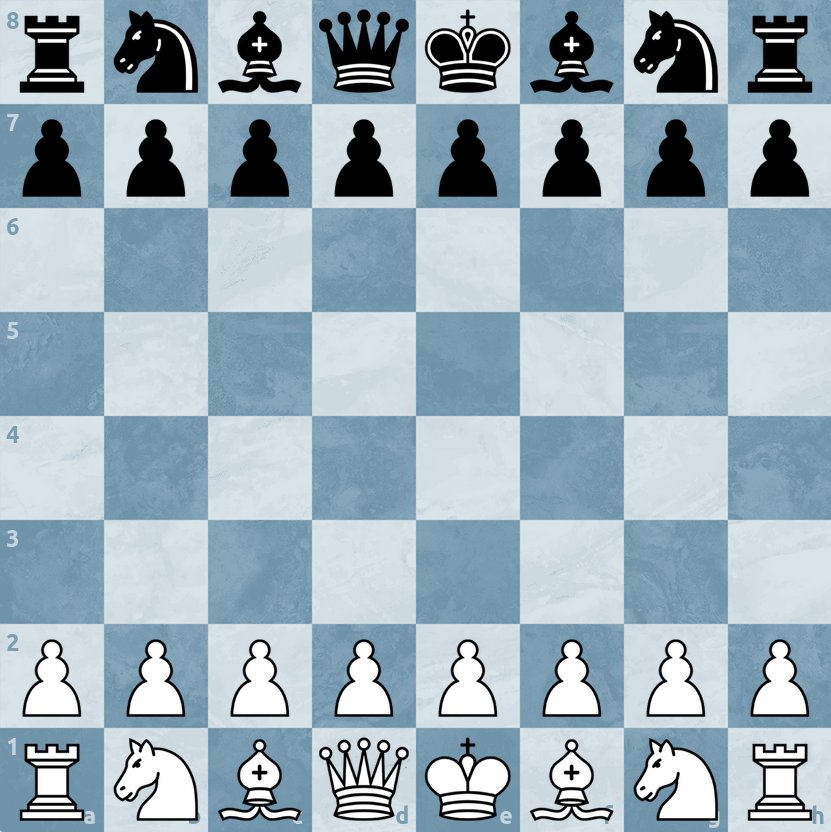
\includegraphics[width=0.6\textwidth]{jeuDepart.png}
    \vspace{0.5cm}
\end{minipage}

Le joueur avec les pièces blanches commence. Ensuite, chaque joueur joue à tour de rôle, un déplacement de pièce par tour.

\subsubsection{Déplacements des Pièces}
Les déplacements sont propres à chaque type de pièce :
\vspace{0.5cm}

\begin{itemize}
    \item \begin{minipage}{0.45\textwidth}
        \textbf{Déplacement du pion :} \\
        Le pion avance uniquement en ligne droite, d'une case à la fois. Toutefois, lors de son premier déplacement, 
        il a la possibilité d'avancer de deux cases. Contrairement à son déplacement habituel, le pion capture les pièces
         adverses en diagonale, en se déplaçant d'une case.
    \end{minipage}
    \hspace{0.05\textwidth}
    \begin{minipage}{0.45\textwidth}
        \centering
        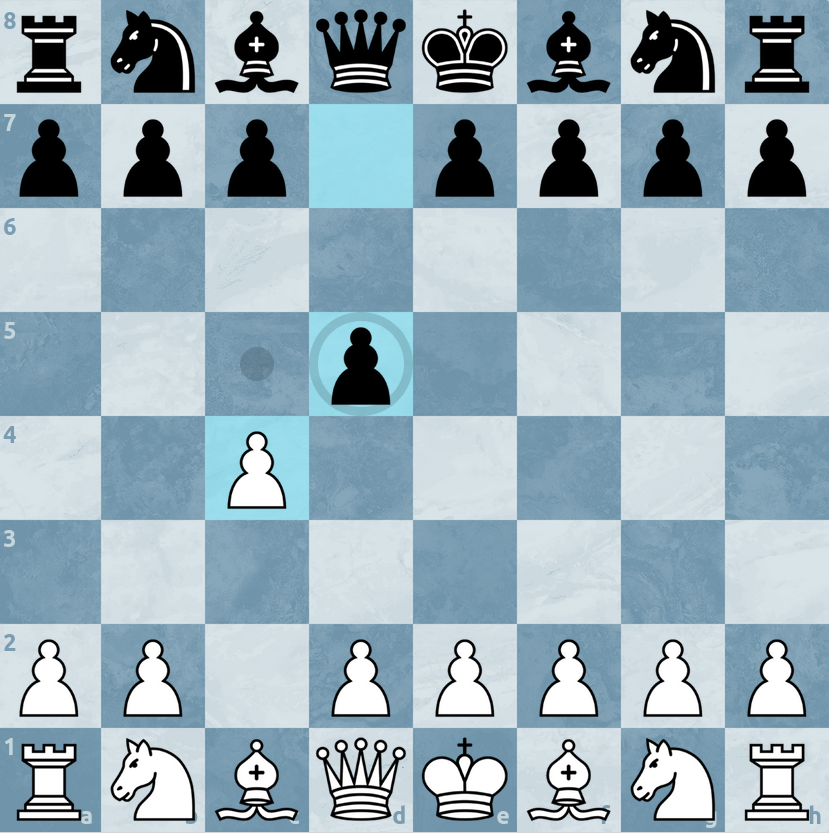
\includegraphics[width=\textwidth]{pionMove.png}
    \end{minipage}

    \vspace{0.5cm}

    \item \begin{minipage}{0.45\textwidth}
        \textbf{Déplacement du cavalier :} \\
        Le cavalier a un déplacement unique en forme de "L", ce qui signifie qu'il se déplace de deux cases dans une direction,
        puis d'une case perpendiculairement (ou inversement). C'est la seule pièce capable de sauter par-dessus d'autres 
        pièces sur l'échiquier.
    \end{minipage}
    \hspace{0.05\textwidth}
    \begin{minipage}{0.45\textwidth}
        \centering
        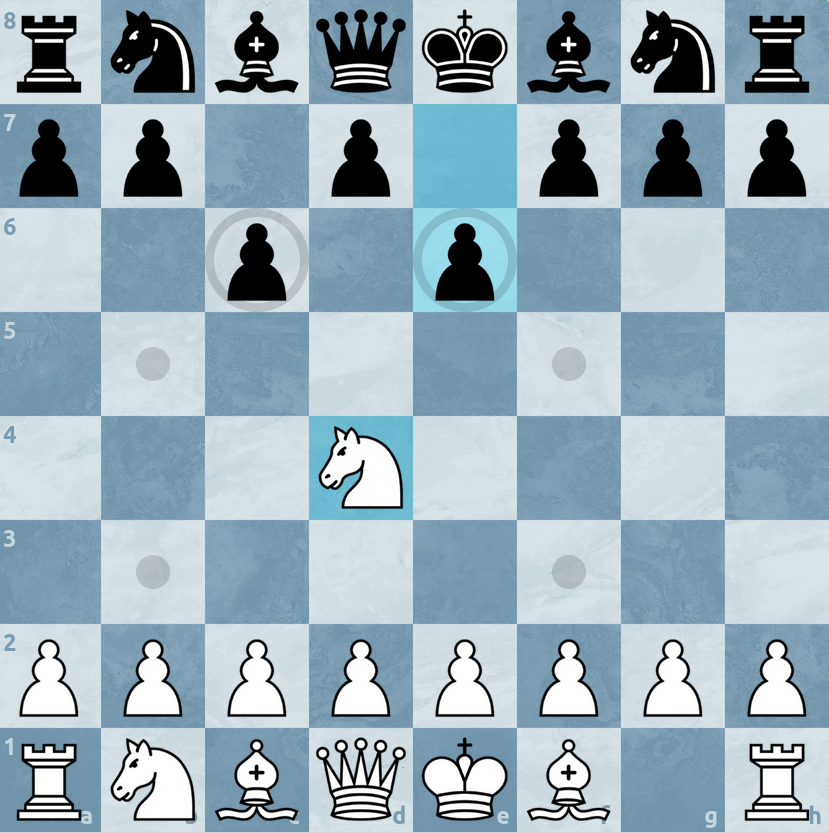
\includegraphics[width=\textwidth]{cavalierMove.png}
    \end{minipage}

    \vspace{0.5cm}

    \item \begin{minipage}{0.45\textwidth}
        \textbf{Déplacement du fou :} \\
        Le fou se déplace en diagonale sur un nombre illimité de cases, tant qu'il n'est pas bloqué par une autre pièce.
         Chaque fou reste toujours sur des cases de la couleur d'où il a commencé (blanches ou noires).
    \end{minipage}
    \hspace{0.05\textwidth}
    \begin{minipage}{0.45\textwidth}
        \centering
        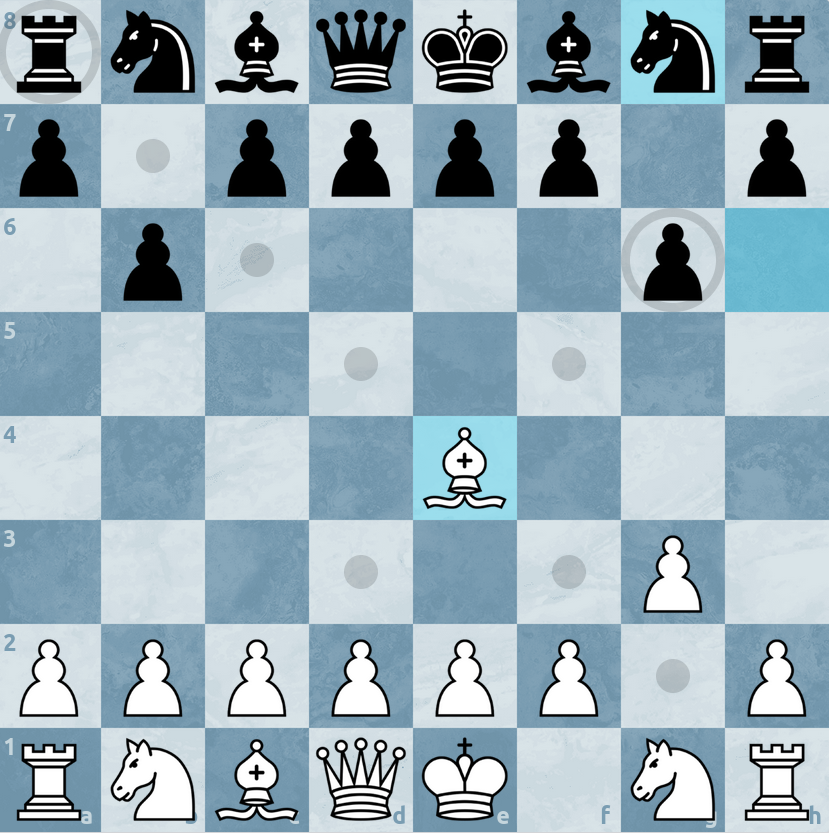
\includegraphics[width=\textwidth]{fouMove.png}
    \end{minipage}

    \vspace{0.5cm}

    \item \begin{minipage}{0.45\textwidth}
        \textbf{Déplacement de la tour :} \\
        La tour peut se déplacer de manière illimitée en ligne droite, que ce soit horizontalement ou verticalement.
        Sa puissance réside dans sa capacité à contrôler des colonnes et des rangées entières.
    \end{minipage}
    \hspace{0.05\textwidth}
    \begin{minipage}{0.45\textwidth}
        \centering
        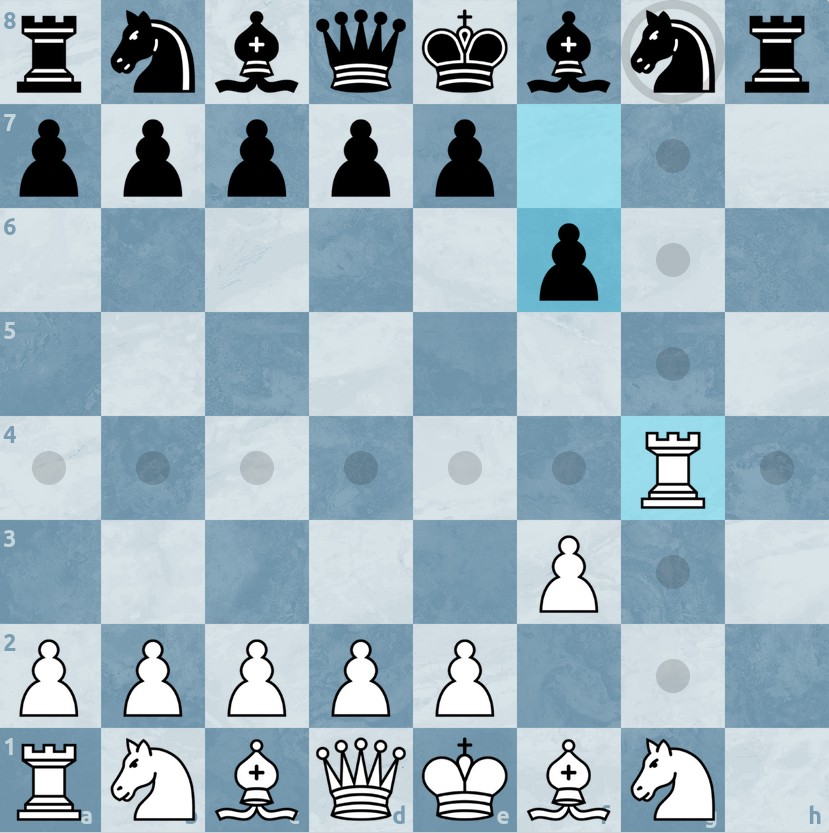
\includegraphics[width=\textwidth]{tourMove.png}
    \end{minipage}

    \vspace{0.5cm}

    \item \begin{minipage}{0.45\textwidth}
        \textbf{Déplacement de la dame :} \\
        La dame est la pièce la plus puissante du jeu. Elle combine les capacités de déplacement du fou et de la tour:
        elle peut se déplacer d'un nombre illimité de cases horizontalement, verticalement ou en diagonale.
    \end{minipage}
    \hspace{0.05\textwidth}
    \begin{minipage}{0.45\textwidth}
        \centering
        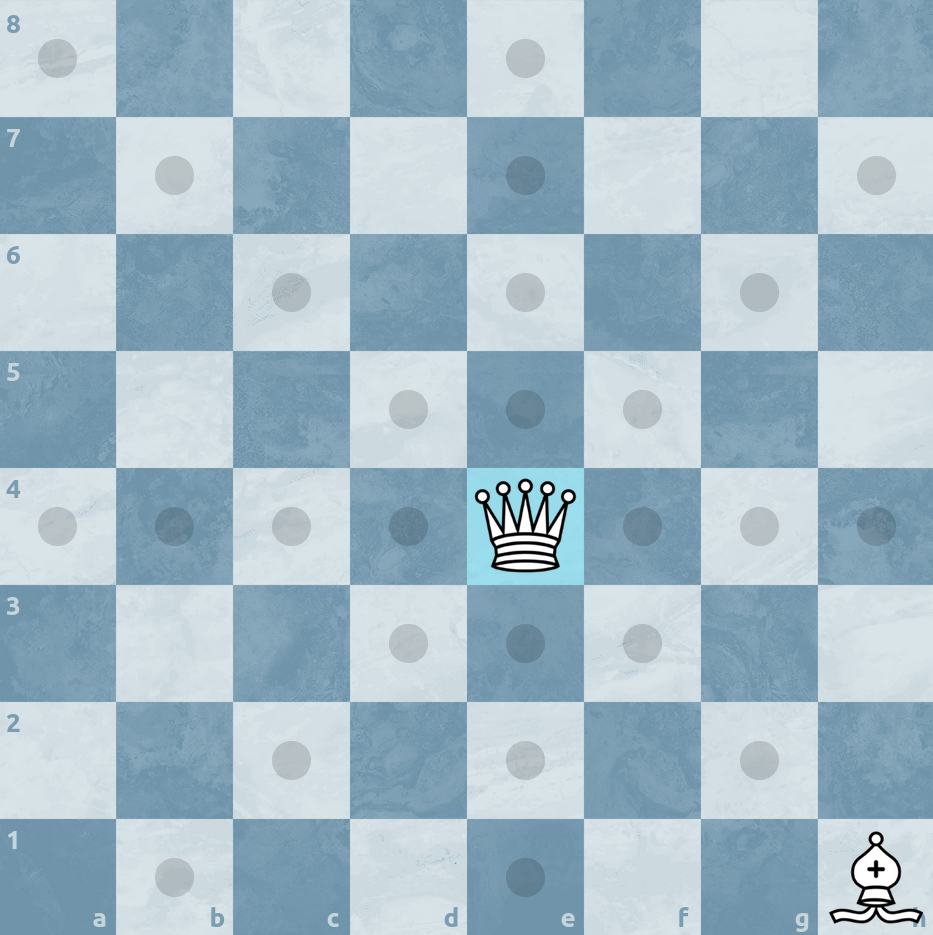
\includegraphics[width=\textwidth]{dameMove.png}
    \end{minipage}

    \vspace{0.5cm}

    \item \begin{minipage}{0.45\textwidth}
        \textbf{Déplacement du roi :} \\
        Le roi peut se déplacer d'une case dans n'importe quelle direction: horizontalement, verticalement ou en diagonale.
        Bien qu'il soit la pièce la plus importante, son mouvement limité le rend vulnérable.
    \end{minipage}
    \hspace{0.05\textwidth}
    \begin{minipage}{0.45\textwidth}
        \centering
        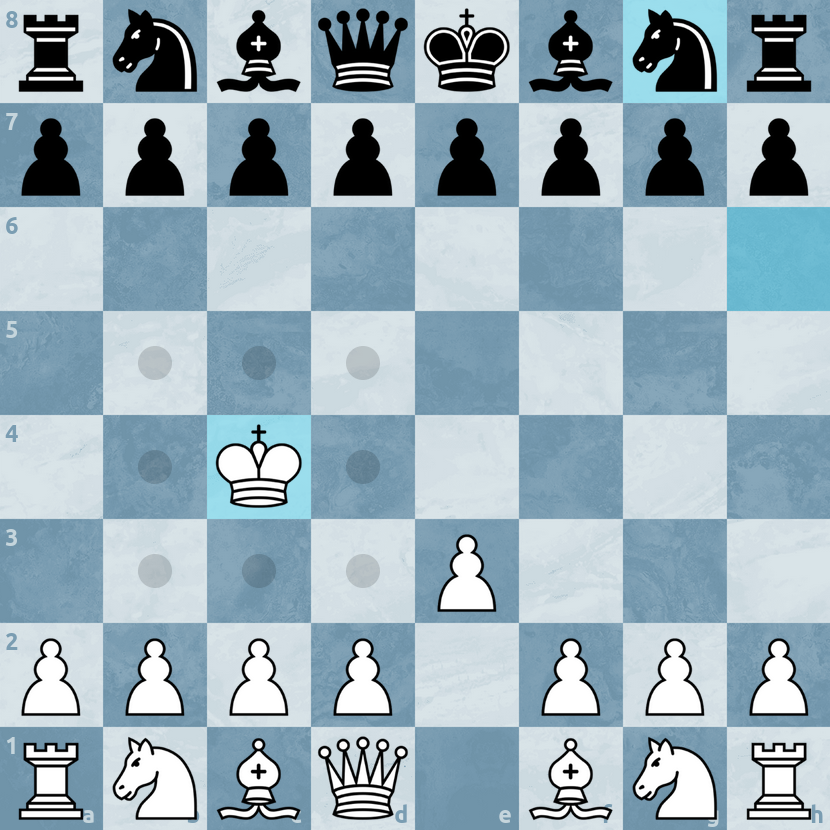
\includegraphics[width=\textwidth]{roiMove.png}
    \end{minipage}

\end{itemize}

\vspace{0.5cm}

Parfois, les déplacements peuvent être limités par des règles spécifiques comme le \textbf{clouage}. Voyons ces règles en détail.

\subsubsection{Règles Spécifiques}
\paragraph{-Clouage} Si une pièce défend une attaque au roi en se positionnant devant cette dernière, on dit qu’elle est \textbf{clouée}
 et ne peut pas bouger. En effet, il est interdit de mettre son roi en échec volontairement par l’une de ses propres actions.

 \noindent
 \begin{minipage}{0.48\textwidth}
     \centering
     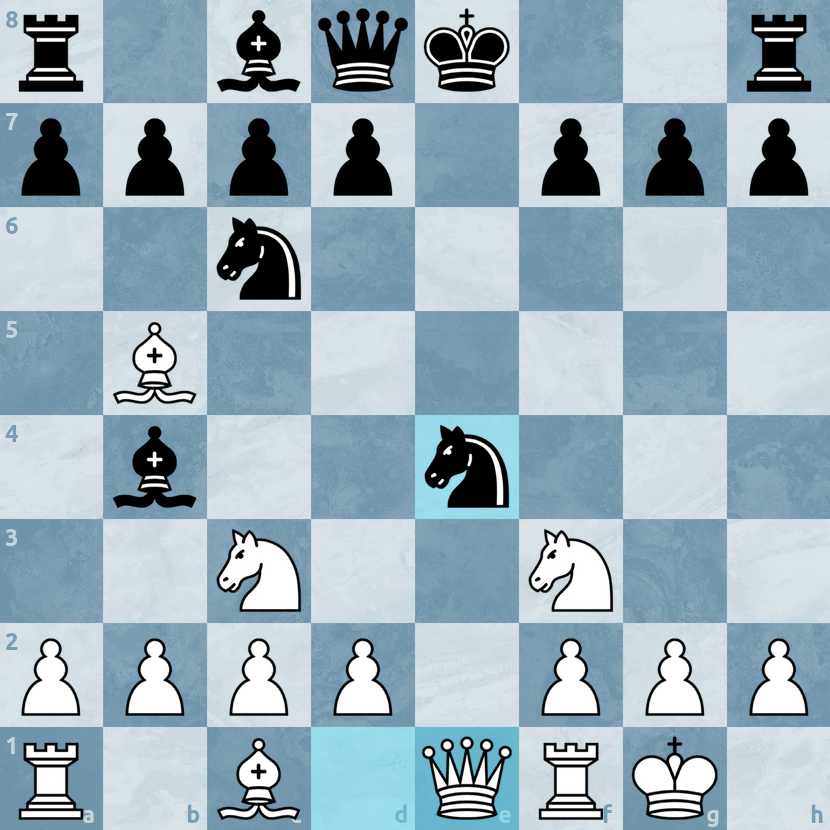
\includegraphics[width=\textwidth, height=\textwidth]{clouage1.png}
     \vspace{0.5cm}
    \textbf{Exemple de clouage}
 \end{minipage}
 \hfill
 \begin{minipage}{0.48\textwidth}
     \centering
     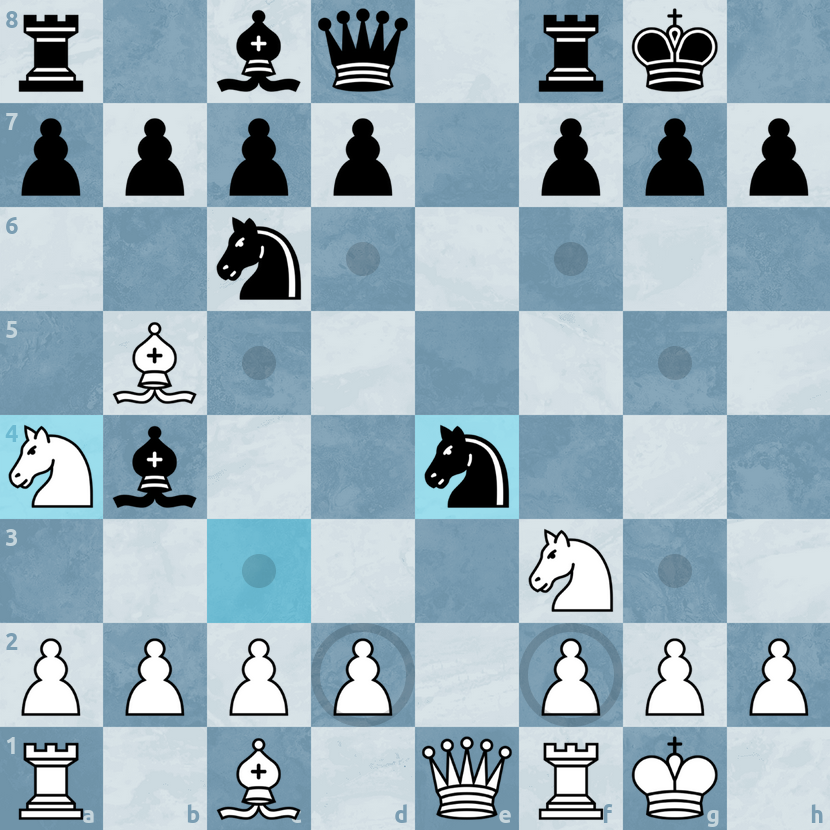
\includegraphics[width=\textwidth, height=\textwidth]{clouage2.png}
     \vspace{0.5cm}
 \end{minipage}

\paragraph{-Roc} Le \textbf{roc} est un mouvement spécial impliquant le roi et une des tours, sous certaines conditions :
\begin{itemize}
    \item Le roi et la tour concernés n’ont jamais bougé depuis le début de la partie.
    \item Le roi ne doit pas être en échec, et aucune des cases qu’il traverse ou sur laquelle il atterrit ne doit être attaquée.
    \item Il ne doit y avoir aucune pièce entre le roi et la tour.
\end{itemize}

\noindent
\begin{minipage}{0.48\textwidth}
    \centering
    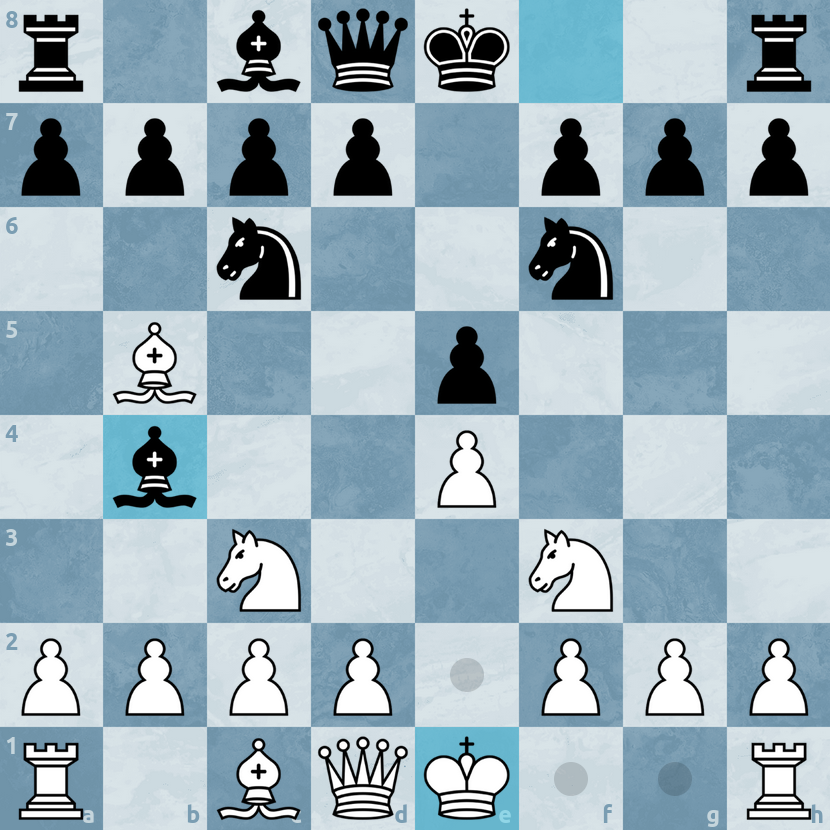
\includegraphics[width=\textwidth, height=\textwidth]{roc1.png}
    \vspace{0.5cm}
   \textbf{Exemple de roc}
\end{minipage}
\hfill
\begin{minipage}{0.48\textwidth}
    \centering
    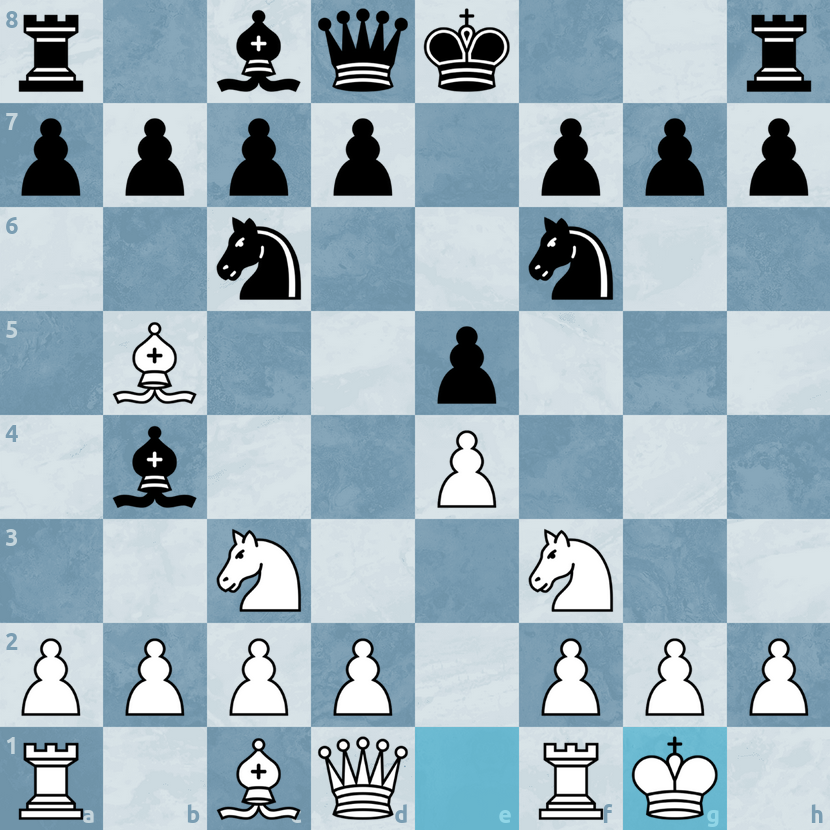
\includegraphics[width=\textwidth, height=\textwidth]{roc2.png}
    \vspace{0.5cm}
\end{minipage}

\paragraph{-Prise en Passant} Si un pion adverse avance de deux cases depuis sa position initiale et finit à côté d’un de nos pions,
 on peut le capturer \textbf{en passant}, mais uniquement au coup suivant.

 \noindent
 \begin{minipage}{0.48\textwidth}
     \centering
     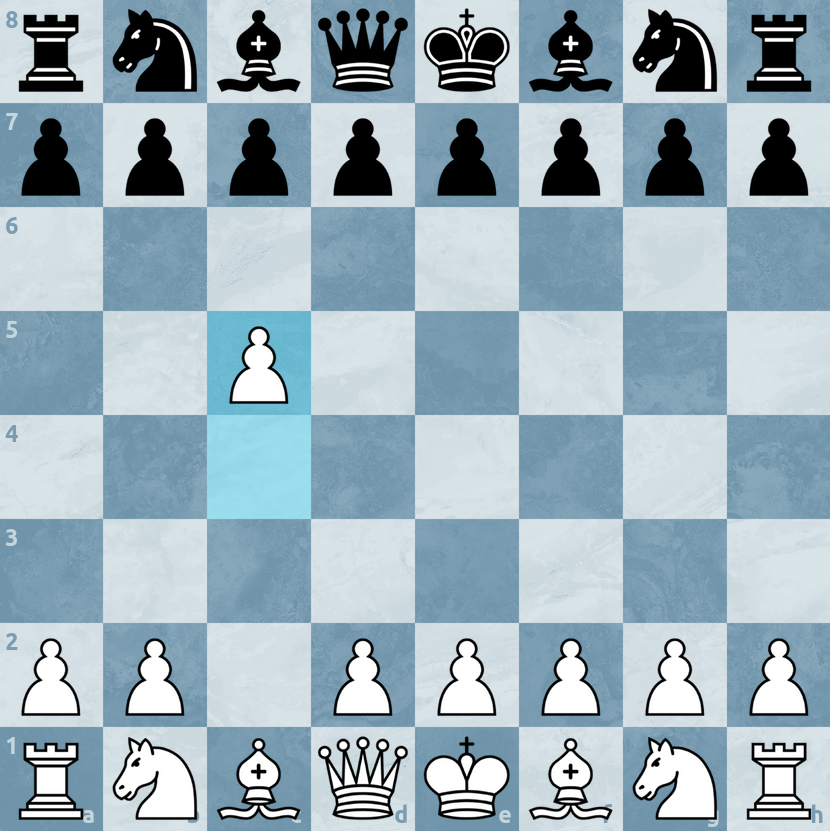
\includegraphics[width=\textwidth, height=\textwidth]{enpassant1.png}
     \vspace{0.5cm}
    \textbf{Exemple de en passant}
 \end{minipage}
 \hfill
 \begin{minipage}{0.48\textwidth}
     \centering
     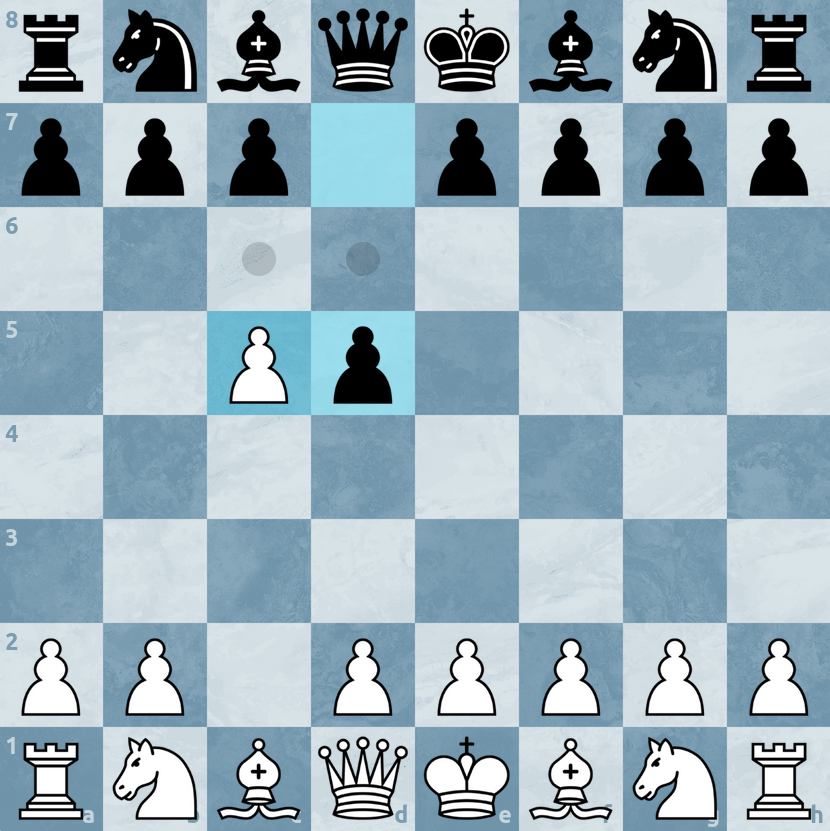
\includegraphics[width=\textwidth, height=\textwidth]{enpassant2.png}
     \vspace{0.5cm}
 \end{minipage}

\paragraph{-Promotion du Pion} Si un pion atteint la dernière rangée de l’échiquier, il peut être promu en dame,
 tour, fou ou cavalier. La promotion du pion est souvent synonyme d’avantage conséquent et peut mener à une victoire.

 \noindent
 \begin{minipage}{0.48\textwidth}
     \centering
     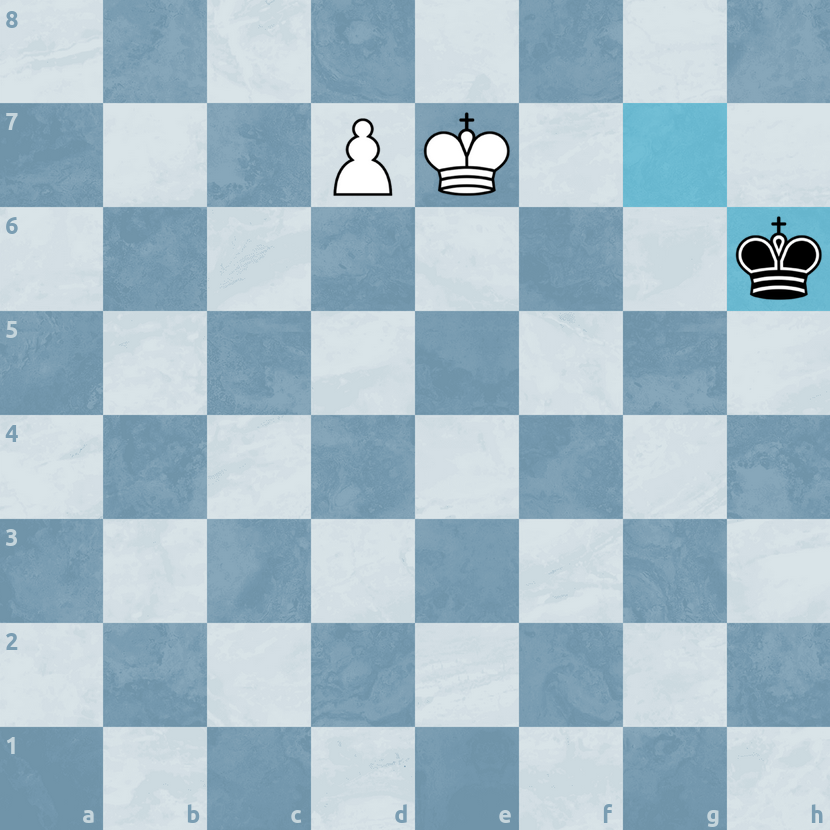
\includegraphics[width=\textwidth, height=\textwidth]{promotion1.png}
     \vspace{0.5cm}
    \textbf{Exemple de promotion}
 \end{minipage}
 \hfill
 \begin{minipage}{0.48\textwidth}
     \centering
     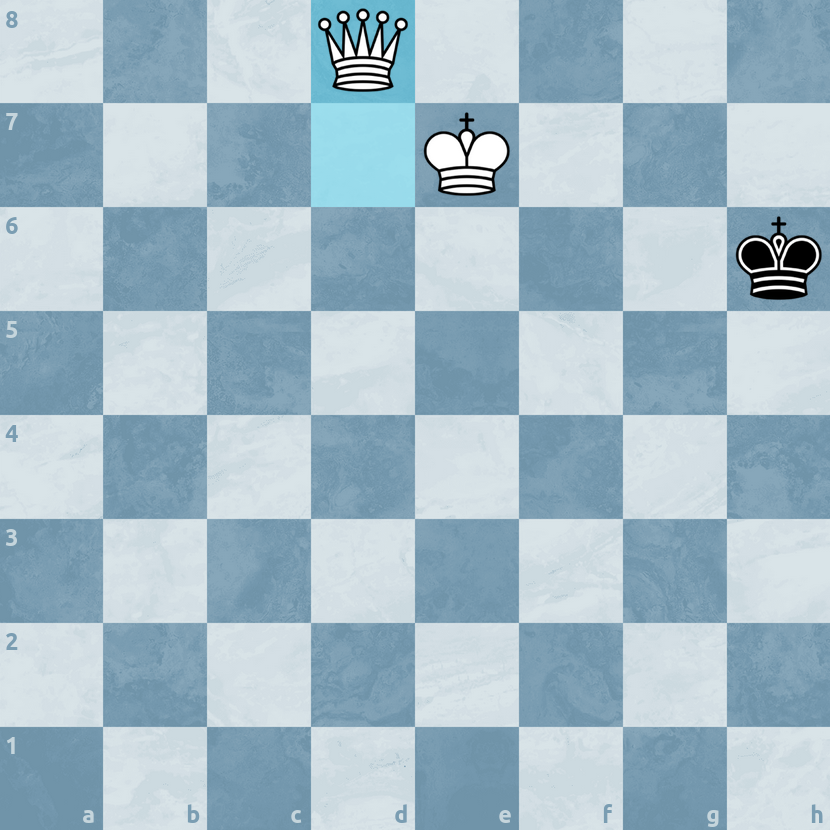
\includegraphics[width=\textwidth, height=\textwidth]{promotion2.png}
     \vspace{0.5cm}
 \end{minipage}

\subsubsection{Fin de Partie}
Une partie d'échecs peut se terminer de plusieurs façons :
\begin{itemize}
    \item \textbf{Échec et mat} : le roi est attaqué et aucun coup légal ne peut le sauver, ce qui donne la victoire à l'adversaire.
    \item \textbf{Pat} : un joueur n’a aucun coup légal à jouer et son roi n’est pas en échec, entraînant une nulle.
    \item \textbf{Manque de matériel} : si seuls les rois, ou un roi et un fou/cavalier, restent sur l'échiquier, un mat devient impossible, ce qui entraîne une nulle.
    \item \textbf{Répétition de position} : une même position exacte apparaît trois fois, entraînant une nulle.
    \item \textbf{Règle des 50 coups} : si aucun pion n’est déplacé ni pièce capturée pendant 50 coups consécutifs, la partie est déclarée nulle.
    \item \textbf{Abandon} : un joueur peut décider d’abandonner si sa position devient trop défavorable.
    \item \textbf{Accord mutuel} : les deux joueurs conviennent de déclarer une nulle lorsqu'aucun ne voit de progrès réaliste possible.
    \item \textbf{Dépassement de temps} : un joueur perd si son chronomètre s’écoule avant qu’il ne joue, sauf si l’adversaire n’a pas assez de matériel pour mater.
\end{itemize}

\subsection{Plateau sous forme de bitmaps}
Un échiquier est finalement une matrice 8x8 (64 cases donc) sur lesquelles il y a une pièce, ou non. On voit ici une
notion de binaire. Pour une pièce: "Blanche ou Noire", "Présente ou Non" (pour les cases). Une méthode existe pour
représenter l'échiquier en se servant de bitmaps plutôt que d'utiliser des arrays, vecteurs ou listes en deux dimensions.
Il s'agit du bitboard. On observera un gain de performance en temps et un gain d'espace énormes pour la représentation
de l'échiquier (et des règles spécifiques).\\
Comment cela va-t-il fonctionner ? Comme on vient de le voir, sur une case, soit il y a une pièce, soit il n'y en a pas.
Encodons le fait qu'une case soit occupée par 1 et le fait qu'une case soit vide (libre) par 0. Il y a 64 cases au total.
Donc, en attribuant un indice à chaque case (de 0 à 63), on va pouvoir chiffrer l'échiquier par un entier de 64 bits.
Chaque bit de cet entier est à 0 ou à 1. S'il est à 0 pour l'indice i, alors la case i est libre. S'il est à 1, alors la
case i est occupée. Un entier n'est cependant pas suffisant, car il faut pouvoir différencier les types de pièce, ainsi
que la couleur des pièces (noire ou blanche). Il y a au total 6 types de pièces aux échecs: le Pion, le Cavalier, le Fou,
la Tour, la Dame, le Roi. Donc finalement, on aura besoin de 12 entiers codés sur 64 bits, car 6 pour les types de pièces
blanches et 6 pour les types de pièces noires.
\\Il est important de noter que cela n'est pas réalisable pour des ordinateurs qui possèdent une architecture en 32 bits.
Aujourd'hui, la quasi-totalité des ordinateurs utilise du 64 bits, donc il ne faut pas trop s'en soucier. C'est néanmoins
crucial de relever les inconvénients des méthodes que l'on va utiliser pour ce projet. Un autre désavantage de cette méthode
est le fait qu'il faudra faire une gymnastique pour "décoder" pour l'humain une position. En effet, si l'on prend l'entier
112, on ne visualise pas (du tout) la position, même si l'ordinateur si.
Retenons aussi que l'on aura à faire à des représentations et opérations binaires, pour lesquelles un ordinateur est très
performant. En Java, chaque entier sera un long (type primitif).
\\Il faut aussi se pencher sur les règles spécifiques que l'on encodera avec les 12 bitmaps pour représenter une position
dans son entièreté. Effectivement, pour le moment, nous n'avons que l'emplacement des pièces sur l'échiquier. Mais une position
est aussi décrite par ses règles, c'est un état de jeu. Les règles à prendre en compte sont:\\
\begin{itemize}
    \item En passant: Il faut utiliser 1 bit comme flag, 1 si en passant possible et 0 sinon. Il y a au total 16 cases cibles où
    un en passant peut se produire. On utilise donc 4 bits (16 valeurs) supplémentaires. Au total donc, 5 bits.
    \item Roques: on compte le grand roque et le petit roque des deux côtés (noirs et blancs). On a donc besoin de 4 bits.
    \item Temps à la pendule: Pour les blancs et les noirs, on doit savoir combien de temps il reste à chaque état du jeu. Si
    l'on se dit que chaque joueur dispose de 24h pour une partie en prenant large, il faut coder 86 400 000 (en ms). Pour cela,
    on a besoin de 27 bits. Mais il s'agit de 27 bits de chaque côté car il y a les blancs et les noirs. Donc au total, 54 bits ici.
    \item Règle des 50 coups: Pour le nombre de coups sans capture ou mouvement de pion, on se sert de 6 bits (entre 0 et 50).
    \item Nombre de "FullMoves": Pour se souvenir du nombre de coups total de la partie, on va prendre large et utiliser 10 bits,
    ce qui nous donne la possibilité d'avoir 1000 coups.
\end{itemize}

Si l'on effectue le total, une position est codée sur 12*64 + 5 + 4 + 54 + 6 + 10 = 847 bits.
C'est un gain très conséquent qui va notamment nous permettre par exemple de chercher à une profondeur plus grande pour la partie
Intelligence Artificielle. Il y a quelques détails en ce qui concerne les performances dans les parties \ref{DataStruct} Structures de données et
\ref{AI} Intelligence Artificielle dans le rapport notamment.

\subsection{Structures de données}
\label{DataStruct}
\subsubsection{Historique des coups}
\par Le groupe s'est posé la question de quelles structures de données utiliser pour stocker l'historique des coups d'une
partie. Il a fallu prendre en compte plusieurs facteurs, notamment la performance, là où les difficultés d'implémentation,
la compatibilité avec les bitboards pour représenter le plateau de jeu, ainsi que les ajouts potentiels de fonctionnalités.
\\La première idée fut une pile. En effet, cette structure est très simple d'utilisation et parfaitement adaptée pour stocker
des coups, tout en ayant la possibilité d'en enlever et d'en rajouter. La complexité en temps et en espace est en O(n) si n 
correspond au nombre de coups de la partie. Pour revenir au tout début de la partie, c'est-à-dire avec les pièces positionnées
sur leurs cases initiales, il suffit de dépiler les n coups stackés en les empiler dans une seconde pile qui s'occupera de sauvegarder
ces coups pour pouvoir revenir au dernire coup joué avant d'avoir repris tous les coups. Ainsi, en utilisant la pile comme structure 
de données, on garde n coups en mémoire, et revenir à une certaine position de la partie est linéaire en fonction de ce nombre de coups.
Avec une interface graphique, on pourrait cliquer sur un certain coup pour savoir combien de coups dépiler, car un coup peut arriver
plusieurs fois dans une partie donc sa représentation ne suffit pas.\\
Cela se présenterait comme ceci:

\begin{figure}[h]
    \caption{Exemple historique de coups}
    \centering
    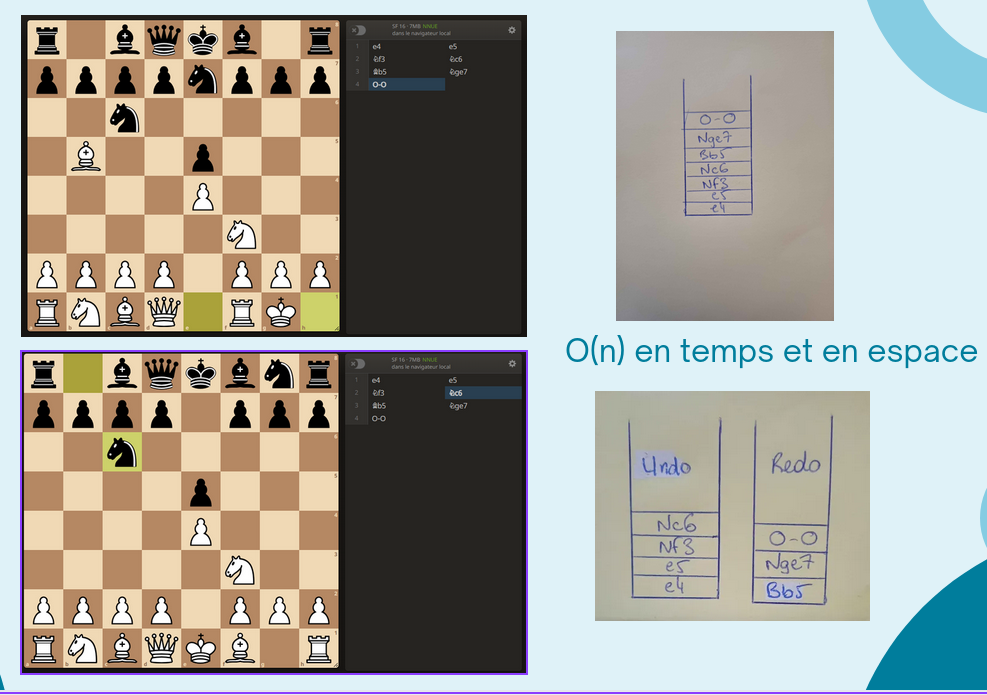
\includegraphics[width=\textwidth,height=6.0cm,keepaspectratio]{pile-historique-coups}
\end{figure}

S'il n'y a pas de fonctionnalité de game review ou de game analysis, et que l'on part du principe qu'il y a écrasement de l'historique
lorsque l'on joue des coups différents de ceux joués initialement, alors la pile est un très bon choix.\\

\par En se projetant, le groupe a réfléchi aux inconvénients de la pile et à l'évolution du projet.
Peut-être est-ce optimiste, mais nous avons prévu deux semaines (deux dernières) pour se pencher vers les améliorations
(fonctionnalités bonus) pouvant être implémentées, ainsi que les aspects qui méritent d'être revus. En particulier, nous avons
pensé à la possibilité de réaliser une game review et/ou une game analysis. Aussi, une fonctionnalité selon laquelle on pourrait 
revenir à une position déjà jouée après avoir joué par dessus des coups repris. En d'autres mots, il n'y aurait pas d'écrasement
(overwritting) des coups.
En prenant cela en compte, il faudrait cette fois utiliser les arbres. En effet, lorsque l'on déroule les branches ou variations de coups,
l'arbre est en fait la structure de données naturelle dont on va se servir.\\
Regardons un exemple pour ensuite discuter les avantages et les inconvénients des arbres:\\
\begin{center}
    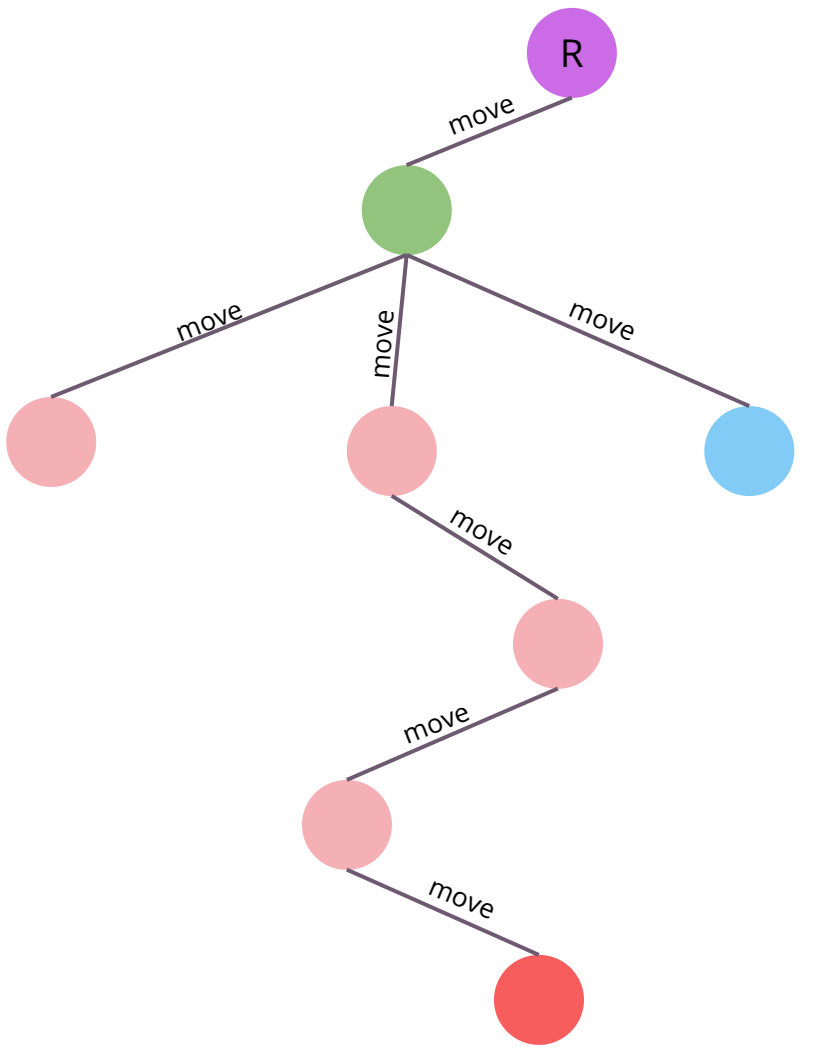
\includegraphics[height=6.0cm]{arbres-branchement-coups.png}
\end{center}

Dans notre exemple, les nœuds représentent les positions
et les arêtes représentent les coups. Si l'on est au nœud rouge, et que l'on souhaite revenir au nœud vert pour aller vers le nœud bleu,
alors la nouvelle branche "main" pour l'historique des coups va du nœud R (Root) jusqu'au nœud bleu. Avant, il allait du nœud R jusqu'au
nœud rouge. \'A chaque nœud de branchement (ici nœud vert), on aurait la possibilité de changer de branche. C'est-à-dire que si l'on revient
au nœud vert, on pourrait retourner au nœud bleu, comme on pourrait retourner au nœud rouge, ou comme on pourrait explorer d'autres coups,
créant ainsi une nouvelle variation depuis ce nœud de branchement.

En terme de performance, au niveau de la complexité en temps, cela serait imbattable, car on pourrait revenir à une position en O(1). En effet,
en se servant d'une Java HashMap\textless Integer, Node\textgreater. On obtiendrait ainsi une référence à partir d'un entier en se servant de
l'interface graphique:\\
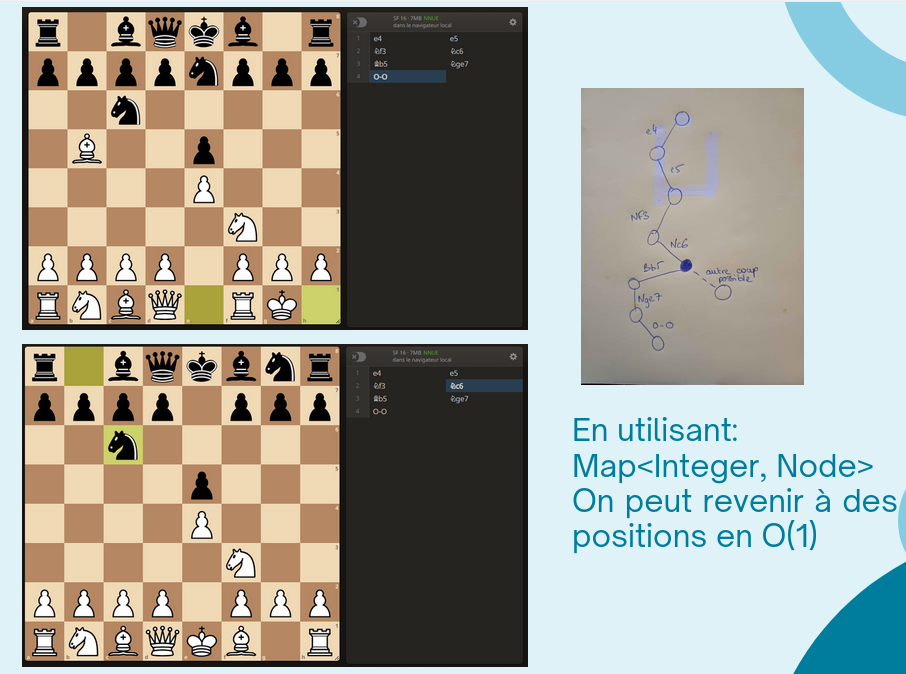
\includegraphics[height=6.0cm]{arbres-reprise-coups.png}

En ce qui concerne la complexité en espace, cela devient un petit peu plus délicat si l'on souhaite être précis. Avant tout, pour permettre de
revenir dans l'ordre en O(1), il faut conserver toutes les références des nœuds de cet arbre. Cela signifie que l'on garde en mémoire n+1 positions 
si n est le nombre de coups joués au total (branches comprises). Comme nous l'avons vu précédemment, une position est encodée par 847 bits.
Finalement, on se retrouve avec une complexité de O(847*n) bits. Pour donner un ordre d'idée, si une partie a enregistré 300 coups, alors en mémoire,
on aura un peu moins de 52KB. Ce n'est donc pas très coûteux en ce qui concerne une partie. En revanche, pour la partie Intelligence Artificielle,
où l'on va tester des milliers de branchements, cela peut devenir assez lourd. Il faudra certainement faire des tests et limiter les opérations
sur ces arbres de jeu afin de ne pas causer de problème.

\par Nous avons donc observé que les arbres sont de manière générale très avantageux dans notre cas, et bien plus que les piles, pour lesquelles
il aurait fallu faire un nombre indécent de copies et donc coûter cher. Même si les variations et game reviews sont hypothétiques, le groupe préfère
ne pas prendre de risque quant à ce choix de structure de données et se servira des arbres pour stocker l'historique des coups d'une partie.
Dans le pire des cas, c'est-à-dire si les game reviews et non-écrasements de l'historique ne sont pas implémentés, l'arbre sera "linéaire"
(degenerate tree) et simulera la pile en conservant les n coups de la partie en mémoire. Donc en espace, nous sommes en O(n).
Néanmoins, en temps, nous sommes toujours en O(1) puisque nous conservons les références vers les nœuds de l'arbre. C'est donc plus efficace que
la pile dans les deux cas, rendant cette approche optimale.

\subsection{Intelligence Artificielle} \label{AI}
\subsubsection{Heuristiques}
Afin de coder une bonne heuristique, aux échecs, il faut prendre en compte beaucoup d'éléments et revenir aux bases du jeu.
Notamment, il faut savoir ce qui importe dans une position, ce qui donne l'avantage ou ce qui assure une égalité. Essentiellement,
on se contente de vérifier certains points clés qui vont nous permettre d'émettre une évaluation sur une position.
Rappelons que le facteur de branchement aux échecs approche les 35.\\
Il y a de nombreux éléments à prendre en compte, et en voici certainement les plus impactants:
\begin{itemize}
    \item Le Matériel: chaque pièce (sauf peut-être le roi) possède une valeur. On va donc s'occuper de compter pour les 2 camps le "potentiel"
    dans une position. Plus on a de matériel (pièces donc), plus on a de chances d'avoir l'avantage, en particulier par un bon contrôle de l'échiquier.
    \item La sécurité du Roi: Le Roi est la pièce la plus importante aux échecs, et souvent, le joueur qui a un avantage est celui qui va
    avoir un Roi qui n'est pas en danger. Pour estimer cela, on peut en particulier vérifier le nombre de coups où l'on peut mettre le Roi en échec,
    combien de coups permettent de l'en sortir, et la fréquence des échecs. Plus un Roi est vulnérable, plus il y aura des possibilités
    de le mettre en échec.
    \item Le contrôle du centre: Aux échecs, le centre est un emplacement clé, puisqu'il peut donner un accès efficace à toutes les parties de
    l'échiquier. Généralement, obtenir un bon contrôle du centre est un facteur qui va jouer dans l'évaluation d'une position.
    \item L'activité: Si l'on a peu de coups légaux que l'on peut jouer, c'est très souvent parce que l'on est en position de désavantage. Cela peut
    signifier que l'on est forcé à jouer certains coups.
    \item La structure de pions: Plus on aura une structure de pions solide, plus on aura de potentiel d'attaque et de défense puisque les pions sont
    des pièces "faibles" lorsqu'ils sont seuls et/ou non défendus.
    \item La promotion: Plus on a de pions avancés, plus on a de chance d'atteindre la dernière rangée et changer notre pion en une pièce plus importante,
    comme la Dame par exemple, nous donnant plus d'options.
\end{itemize}

Seulement ceux-là sont cités ici, mais en réalité, il y a plus de 20 points clés nous permettant d'évaluer une position de manière efficace.
Enfin, afin d'obtenir une bonne heuristique aux échecs, il faut considérer tous ces points et faire une somme. Puisque c'est un jeu à somme nulle,
c'est la marche à suivre. 

\subsubsection{Algorithmes}
Dans cette partie Intelligence Artificielle, on va essentiellement se servir des 3 algorithmes suivants (dont 2 vus au dernier semestre):
\begin{itemize}
    \item MiniMax: Visant à retourner l'option la plus adéquate dans une certaine position, on utilise des arbres pour savoir quelle branche va être la
    plus intéressante, que ce soit pour l'ami, comme pour l'ennemi. On est en O($b^d$) en temps, où b est le facteur de branchement et d la profondeur.
    En espace, c'est du O(d), soit le nombre de niveaux dans l'arbre pour une approche basée sur du DFS.
    \item AlphaBeta-pruning: Cet algorithme se repose sur MiniMax, mais peut permettre d'aller à une profondeur deux fois plus grande si les nœuds de
    l'arbre sont organisés du plus petit au plus grand. Ici, la valeur des nœuds va être une évaluation. La complexité en espace ne change pas, mais
    en temps nous sommes donc en O($b^p$) où p = d/2.
    \item Monte Carlo Tree Search: Celui-ci peut se décomposer en quatres étapes: "Selection","Expansion","Simulation","BackPropagation". Pour faire simple,
    on va choisir (Selection) des branches à explorer. Cela peut être les nœuds qui vont être impactants sur la recherche du meilleur coup,
    ou encore des nœuds qui n'ont pas encore été explorés. Ensuite, après avoir choisi la branche, on se positionne à la feuille de cette branche,
    puis on simule un coup aléatoirement (Expansion) et on l'évalue. Maintenant, à partir de ce nouveau nœud, on simule une partie ou une pseudo-partie
    aléatoirement pour estimer le résultat potentiel. Finalement, lorsque l'on obtient un résultat, on fait remonter l'évaluation (BackPropagation)
    et/ou les informations importantes vers le haut de l'arbre pour plus tard agir en conséquence. En temps, on se rapproche de O(n*d), où n est le
    nombre de simulations effectuées, et d la profondeur moyenne. En espace, on est en O(n*847) où n est le nombre de nœuds au total, et 847 le
    nombre de bits (la taille) d'un nœud.
\end{itemize}

\par Notons que tous les algorithmes s'effectuent sur des arbres et se servent d'une heuristique pour évaluer chaque position. Pour optimiser ces algorithmes, 
on utilisera surtout deux techniques: le Forward-prunig et la Reduction.

\subsection{Zobrist hashing} \label{Zobrist}
Le hachage Zobrist est une fonction utilisée en particulier dans les jeux comme les échecs ou le go, où le but est d'attribuer un codage "complexe" à
une position, pour éviter d'analyser une position plus d'une fois. Ainsi, on peut gagner en performance, notamment dans les algorithmes d'IA, où les
états de jeu peuvent se répéter un grand nombre de fois. On va se servir de ce qu'on appelle des "tables de transposition", qui sont des tables de
hachage indexées par une position. Comment cela fonctionne-t-il ? Dans notre cas, les positions sont encodées par 12 bitmaps, et quelques bits
supplémentaires pour les règles spécifiques. Pour chaque combinaison case-pièce, on va générer un nombre aléatoire. De cette façon, toutes les configurations
de plateaux vont être rencontrées. Le hachage va consister à combiner toutes ces chaînes de bits pour chaque configuration avec l'opérateur XOR,
pour à la fin obtenir un hachage final pour chaque position. Ainsi, en utilisant une HashMap, on va conserver tous les hachages représantant toutes les
configurations possibles pour les utiliser plus tard. Par exemple, pour la règle "Threefold repetition", il faut vérifier si dans cette table de hachage
il existe un hachage H tel que H >= 3. Si c'est le cas, alors la partie se termine en égalité.
\\Donc, dans notre cas, on aura quelque chose de la sorte:\\
\begin{itemize}
    \item ZobristBoardTable[64][12]
    \item ZobristEnPassantTable[64]
    \item ZobristCastlingRightsTable[16]
    \item ZobristFiftyMoveRuleTable[51]
    \item ZobristFullMoveTable[1025]
\end{itemize}

\par Chaque élément sera donc en premier aléatoire, puis bits à bits, des opérations avec XOR seront réalisées. C'est avantageux car lorsque l'on joue
un coup, donc que l'on change l'état du jeu, il n'y a pas à tout recalculer. D'abord, on XOR le nombre aléatoire correspondant à la pièce qui quitte
sa case de départ, puis celui pour la case d'arrivée de cette pièce, et éventuellement changer les bits pour les règles spécifiques.
Pour l'IA, cette méthode sera clé car elle fera gagner en performance, car les états de jeu peuvent se répéter un grand nombre de fois (même si pas
toujours dans le même ordre).

\section{Besoins visés}
\subsection{Quels besoins ?}
Dans le sujet donné, il y avait une liste de 60 besoins.
Nous avons pris la décision ambitieuse de répondre à tous ces besoins. C'est un travail conséquent,
mais avec une équipe de 5 personnes, codant pendant huit semaines,
nous pensons que cet objectif est atteignable.

Nous avons tout de même classé ces besoins par ordre de priorité (voir \nameref{agenda}), afin de garantir
la jouabilité projet même si nous n'arrivons pas à tout implémenter à temps.
Nous voulons rendre un jeu cohérent et fonctionnel avec des modules entièrement
terminés (même s'il en manque) plutôt qu'un projet avec des règles manquantes,
une intelligence artificielle bâclée et une interface graphique peu fonctionnelle.

\subsection{Dépendances entre les besoins}
\subsubsection{Gestion des options}
La première dépendance que nous avons concerne la gestion des options (Figure \ref{fig:needs_options}).

\begin{figure}[h]
    \caption{Besoins concernant la gestion d'options}
    \centering
    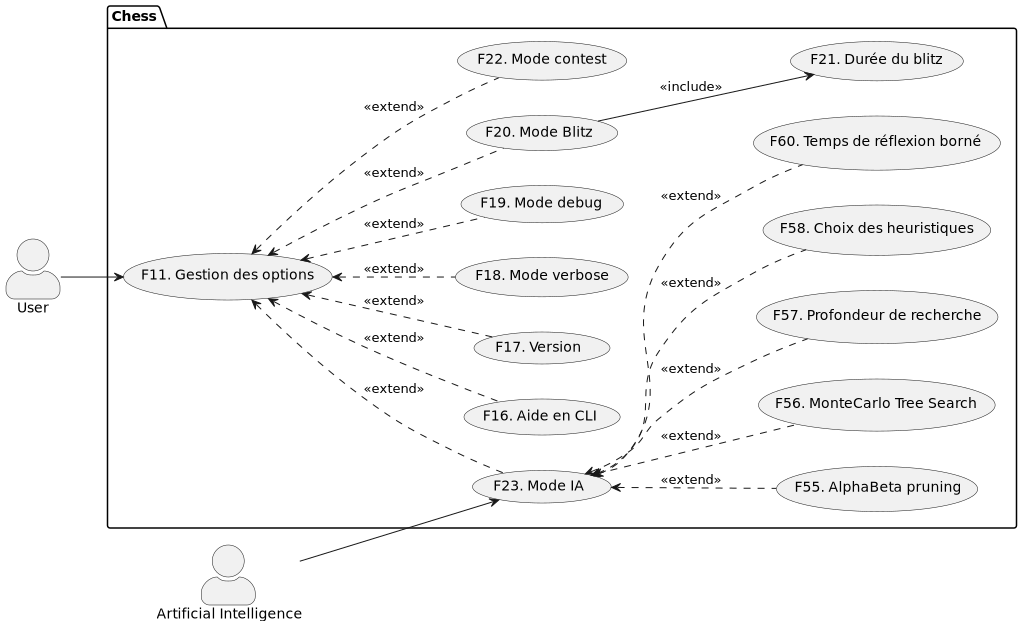
\includegraphics[width=\textwidth,height=\textheight,keepaspectratio]{needs_options}
    \label{fig:needs_options}
\end{figure} 

L'implémentation de la \textit{gestion des options }permettra de rajouter de nombreuses fonctionnalités.
En effet, ceci nous permettra d'implémenter le Mode contest, la version du jeu ou l'aide en ligne de commande. Nous pourrons également gérer les messages affichés grâce au mode verbose ou au mode debug.
Lorsque cela sera implémenté, l'utilisateur aura également le choix entre afficher le jeu en ligne de commande ou avec une interface graphique.
Le mode Blitz inclura le besoin Durée du blitz afin de paramétrer ce mode.
Le mode IA, qui a besoin de la gestion des options, possède quant à lui de nombreuses extensions. En effet, nous pourrons paramétrer
notre intelligence artificielle grâce à d'autres options, que nous verrons cela plus en détail à la section \ref{IA}.


\subsubsection{Sauvegarde de l'historique}
La gestion de l'historique est un besoin indispensable pour notre jeu (Figure \ref{fig:needs_files}).
Beaucoup de besoins dépendent de cette fonctionnalité.
\begin{figure}[h]
    \caption{Besoins concernant la sauvegarde de l'historique}
    \centering
    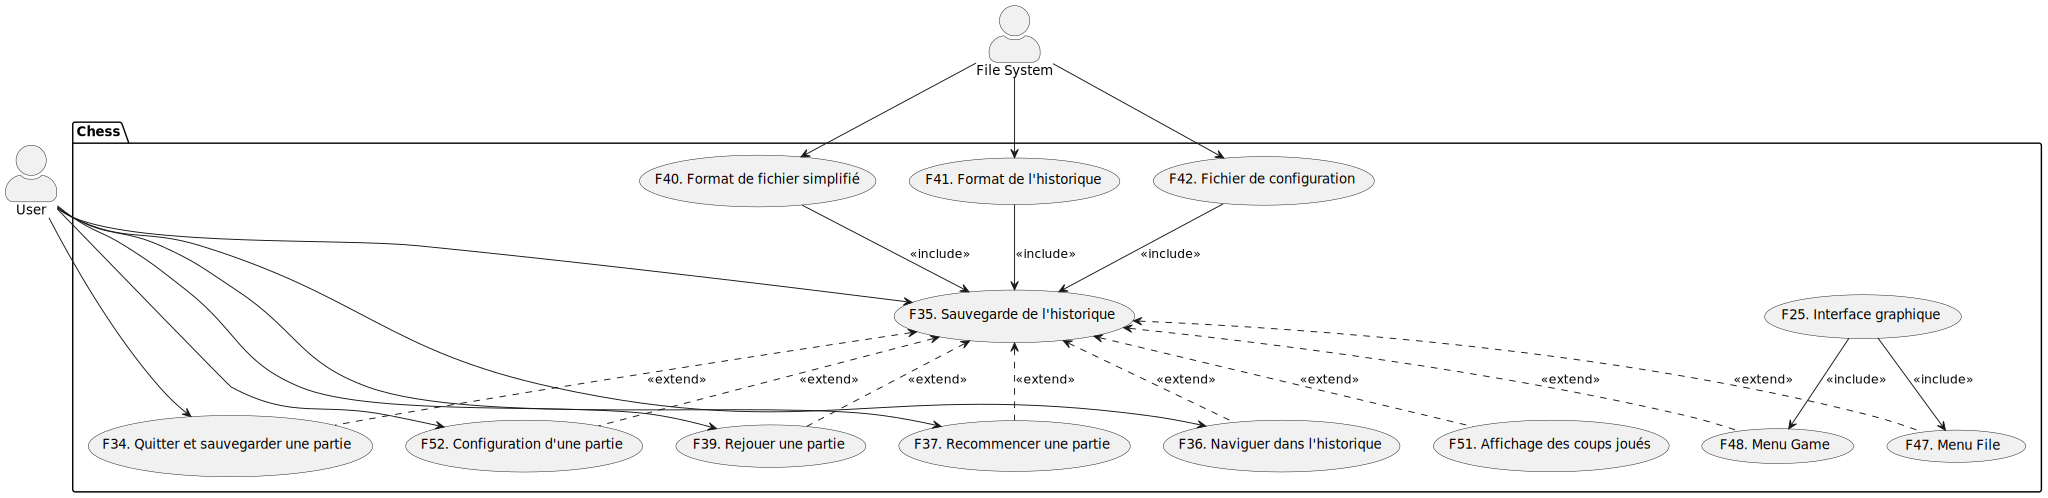
\includegraphics[width=\textwidth,height=\textheight,keepaspectratio]{needs_files}
    \label{fig:needs_files}
\end{figure}

Avant de pouvoir implémenter la gestion de l'historique, il faudra d'abord choisir les formats de fichiers.
Pour cela, il faudra remplir les besoins suivants: \textit{Format de fichier simplifié}, \textit{Format de l'historique} et \textit{Fichier de Configuration}.
Une fois ces besoins implémentés, la sauvegarde de l'historique sera donc possible.
Des besoins utiles au bon déroulement du jeu en dépendent. Grâce à cela, l'utilisateur pourra sauvegarder
sa partie, rejouer ou recommencer une partie. Il pourra également configurer sa partie en modifiant les données du fichier de configuration.
Cela permettrait aussi d'afficher les coups précédemment joués, et même de remonter dans l'historique pour annuler un coup et revenir en arrière.
Certains menus de l'interface graphique permettront également de gérer ces fichiers de sauvegarde et de configuration (voir figure \ref{fig:needs_gui}).

\subsubsection{Intelligence artificielle}
\label{IA}
L'implémentation d'une intelligence artificielle est un autre besoin central du jeu. En effet, cela pourra
permettre à l'utilisateur de jouer contre une machine. Cela pourrait également permettre de donner des
indications sur les meilleurs coups à jouer pour le joueur.

\begin{figure}[h]
    \caption{Besoins concernant l'intelligence artificielle}
    \centering
    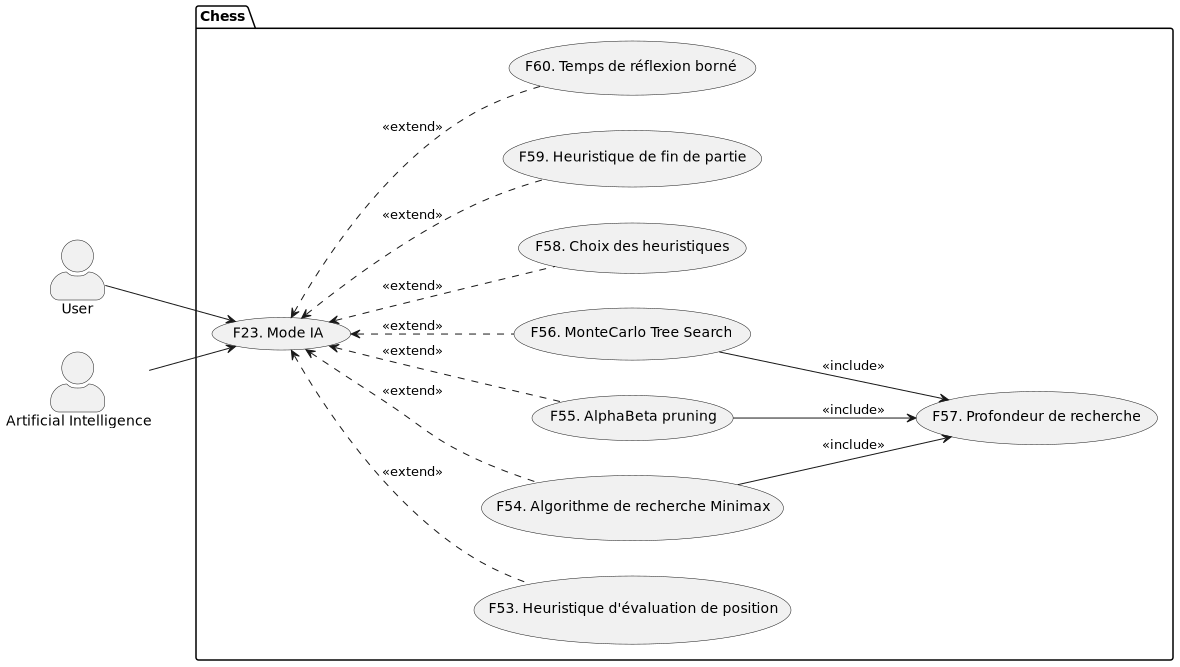
\includegraphics[width=\textwidth,height=\textheight,keepaspectratio]{needs_ai}
    \label{fig:needs_ai}
\end{figure}

Comme affiché Figure \ref{fig:needs_ai}, nous pouvons voir que de nombreux besoins
concernent l'intelligence artificielle.
La plupart des besoins affichés sont également présent dans la Figure \ref{fig:needs_options}, car ils sont paramétrables
en ligne de commande.
Le mode IA contient différentes fonctionnalités concernant les heuristiques. Nous devons implémenter différentes \textit{heuristiques}
d'évaluation de position, mais également au moins une heuristique de fin de partie. Ces heuristiques permettront "d'aider" le joueur IA
à jouer. Ces heuristiques pourront être utilisées avec l'\textit{algorithme de recherche Minimax} mais également lors de l'\textit{AlphaBeta pruning} 
et le \textit{Monte Carlo Tree Search}. Ces algorithmes dépendent tous de l'option \textit{Profondeur de recherche}. En effet, le jeu des échecs est bien 
trop complexe pour simuler une partie entière, et nous devons nous limiter à une certaine profondeur de recherche (nombre de coups à jouer puis analyser).
Borner le temps de "réflexion" de l'IA est aussi un moyen de limiter les calculs de ces algorithmes. Cela pourrait permettre à l'utilisateur de jouer une partie contre
un joueur IA plus ou moins efficace ou d'attendre plus ou moins longtemps entre ses tours.
\subsubsection{Interface graphique}
Les derniers besoins que nous avons rassemblés sont ceux concernant l'interface graphique (Figure \ref{fig:needs_gui}).
\begin{figure}[h]
    \caption{Besoins concernant l'interface graphique}
    \centering
    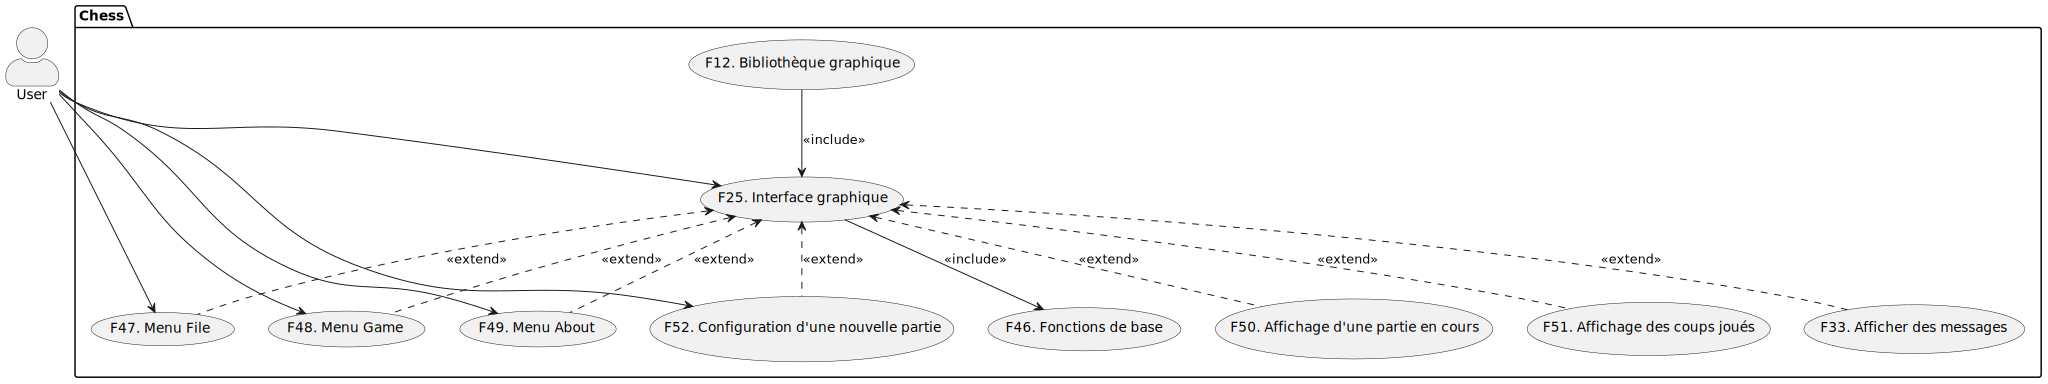
\includegraphics[width=\textwidth,height=\textheight,keepaspectratio]{needs_gui}
    \label{fig:needs_gui}
\end{figure}

L'interface graphique dépend de la \textit{bibliothèque graphique} choisie, ici elle est imposée, il s'agit de \textit{JavaFX}.
L'utilisateur peut choisir de l'utiliser grâce aux options en ligne de commande (Figure \ref{fig:needs_options}).
Elle doit permettre d'utiliser les fonctions de base que nous avons implémenté pour le jeu en ligne de commande. Nous devons 
pouvoir afficher la partie en cours, les coups joués, ainsi que des messages selon le mode utilisé (Verbose ou Debug, voir figure \ref{fig:needs_options}).
L'utilisateur doit également pouvoir utiliser différents menus afin de pouvoir paramétrer ou sauvegarder sa partie (voir figure \ref{fig:needs_files}) ou obtenir des informations sur le jeu.

\section{Agenda prévisionnel}
\label{agenda}

Nous avons décidé de séparer le temps de programmation en quatre parties. Les trois premières seront rythmées besoin par besoin, et la dernière quant à elle sera dédiée à la finalisation du projet et la préparation d'un livrable.
Une partie des besoins sera également suivie tout au long du projet afin de maintenir une base cohérente.

\subsection{Tout au long du projet}

Gestion des aspects fondamentaux et comme le style de codage, les tests, les performances, et la documentation pour garantir la cohérence et la qualité globale du code.

\begin{itemize}
    \item F1. Langage de programmation
    \item F2. Style de codage
    \item F3. Langue par défaut dans le code
    \item F4. Système cible
    \item F5. Documentation
    \item F6. Tests
    \item F10. Frameworks de tests
    \item F7. Bugs
    \item F8. Performances
    \item F9. Build-system
    \item F14. Nom de l’exécutable principal
    \item F15. Usage général
\end{itemize}

\subsection{Semaines 0-2}

Mise en place des fonctionnalités essentielles pour le jeu en ligne de commande, telles que la gestion des options CLI, les règles de jeu, et l'affichage de l'échiquier.

\begin{itemize}
    \item \textbf{Options CLI :}
    \begin{itemize}
        \item F11. Gestion des options
        \item F16. Aide en ligne de commande
        \item F17. Version
        \item F18. Mode verbose
        \item F19. Mode debug
        \item F13. Internationalisation
    \end{itemize}
    \item \textbf{Gestion du jeu :}
    \begin{itemize}
        \item F43. Plateau de jeu
        \item F44. Module bitboard
        \item F45. État du jeu
    \end{itemize}
    \item \textbf{Règles :}
    \begin{itemize}
        \item F29. Prise en passant
        \item F30. Roque
        \item F31. Promotion du pion
        \item F38. Fin de partie
    \end{itemize}
    \item \textbf{Jeu CLI :}
    \begin{itemize}
        \item F24. Interface en ligne de commande
        \item F26. Affichage de l’échiquier
        \item F27. Notation des coups
        \item F28. Représentation de l’historique
        \item F33. Affichage des messages
    \end{itemize}
\end{itemize}

\subsection{Semaines 2-4}

Développement de l'IA, avec des algorithmes comme Minimax et Monte Carlo, et ajout de fonctionnalités avancées comme la sauvegarde, la navigation dans l'historique, et le fichier de configuration.

\begin{itemize}
    \item \textbf{IA :}
    \begin{itemize}
        \item F23. Mode IA
        \item F53. Heuristique d’évaluation de position
        \item F54. Algorithme de recherche Minimax
        \item F55. $\alpha\beta$-pruning
        \item F56. Monte Carlo Tree Search
        \item F57. Profondeur de recherche
        \item F59. Heuristique de fin de partie
        \item F60. Temps de réflexion borné
    \end{itemize}
    \item \textbf{Fonctionnalités :}
    \begin{itemize}
        \item F32. Abandon
        \item F34. Quitter et sauvegarde une partie
        \item F35. Sauvegarde de l’historique
        \item F36. Naviguer dans l’historique
        \item F37. Recommencer une partie
        \item F40. Format de fichier simplifié
        \item F41. Format de l’historique
        \item F42. Fichier de configuration
    \end{itemize}
\end{itemize}

\subsection{Semaines 4-6}

Création de l'interface graphique et finalisation des fonctionnalités utilisateurs, incluant les menus interactifs, la gestion des parties, et les modes spéciaux comme le mode blitz et contest.

\begin{itemize}
    \item \textbf{Interface graphique :}
    \begin{itemize}
        \item F12. Bibliothèque graphique
        \item F25. Interface graphique
        \item F46. Fonctions de base
        \item F47. Menu ’File’
        \item F48. Menu ’Game’
        \item F49. Menu ’About’
        \item F50. Affichage d’une partie en cours
        \item F51. Affichage des coups joués
        \item F52. Configuration d’une nouvelle partie
    \end{itemize}
    \item \textbf{Fonctionnalités :}
    \begin{itemize}
        \item F20. Mode blitz
        \item F21. Durée du blitz
        \item F22. Mode contest
        \item F39. Rejouer une partie
        \item F58. Choix des heuristiques
    \end{itemize}
\end{itemize}

\begin{figure}[h]
    \caption{Diagramme de Gantt (draft)}
    \centering
    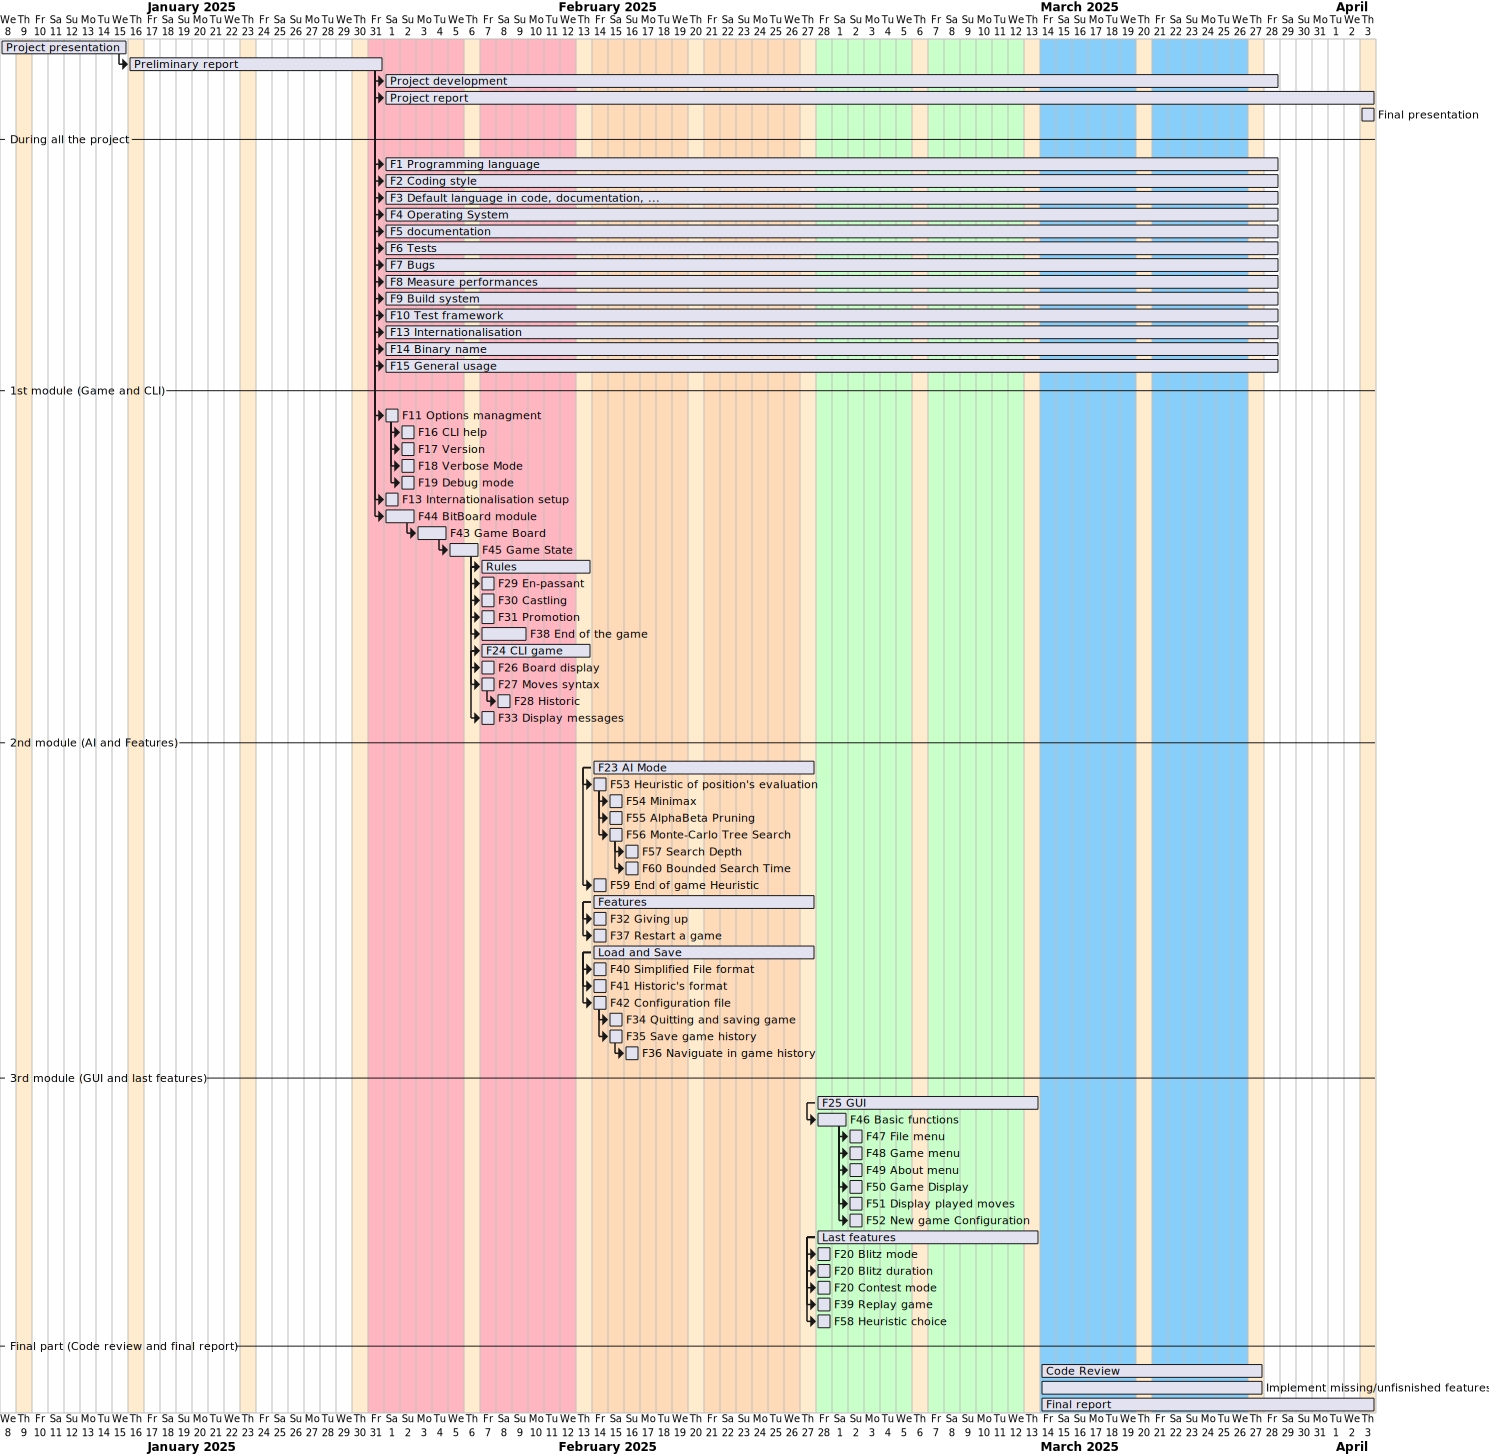
\includegraphics[width=\textwidth,height=\textheight,keepaspectratio]{gantt}
    \label{fig:gantt}
\end{figure}

Le diagramme de Gantt (figure \ref{fig:gantt}) schématise notre agenda prévisionnel. Il n'est pas dans sa version définitive, car nous n'avons
pas encore fait les spécifications étendues.

\section{Architecture visée pour le projet}
Nous avons décidé de présenter le projet sous une forme d'architecture MVC personnalisée. Cette architecture est particulièrement pratique pour nous, développeurs, aussi bien en termes de maintenance que pour l'amélioration future du projet.

Les différents modules de notre projet sont les suivants : \textbf{Model}, \textbf{Controller}, \textbf{Vue}, \textbf{Events} et \textbf{Utils}. 

Voici l'architecture UML du projet : 

\begin{verbatim}
"@startuml
top to bottom direction

package "Model" #DDDDDD{
    class Game {
        - Timer timeWhite
        - Timer timeBlack
        - boolean isTimed
        - Board board
        - History history
        - Solver solver
        + boolean isOver()
        + String getStringHistory()
        + List<Move> getMovesHistory()
    }

    class History {
        - Tree<HistoryNode> tree
        - HistoryNode currentState
        + Move getPrevious()
        + List<Move> getNext()
        + addMove()
        + setCurrent(HistoryNode)
    }

    class HistoryNode {
        - Board state
        - Move previousMove
        - HistoryNode parent 
        - List<HistoryNode> children
        + addChildren(HistoryNode)
    }

    class Board {
        - Bitmap[12] board
        - boolean player
        - boolean enPassant
        + List<Move> getAvailableMoves()
        + boolean makeMove(Move move)
        + Board getCopy()
        + boolean isAttacked(int i, int j)
        + boolean isCheck()
        + boolean isCheckMate()
        + String getPieceAt(int i, int j)
    }

    class Bitboard {
        - long board
    }

    class Move {
        - String move
        + Piece getPiece()
        + getOriginalCol()
        + getOriginalRow()
        + getTargetCol()
        + getTargetRow()
        + Move getReverse()
        + String toString()
    }

    interface Piece {
        + List<Move> getAvailableMoves(boolean isWhite, Board b, int col, int row)
    } 

    class Pawn {}
    class King {}
    class Queen {}
    class Rook {}
    class Bishop {}
    class Knight {}
    
    class Timer {
        - double timeRemaining
        + addTime(double time)
        + startTimer()
        + stopTimer()
    }
}

package "View" #DDDDDD{
    interface Vue{
    + movePlayed()
    + pieceTaken()
    + displayBoard()
    + onGameEnd()
    }
    class CLIVue
    class GameVue
}

package "Controller" #DDDDDD{
    class GameController {
        - Vue vue
        - Game model
        + void handleEvent(GameEvent event)
    }
}

package "Events" #DDDDDD{
    class EventSource {
        - List<GameEventObserver> observers
        + void addObserver(GameEventObserver observer)
        + void removeObserver(GameEventObserver observer)
        + void notifyObservers(GameEvent event)
    }

    class GameEvent {
        - GameEventType eventType
        - Object data
        + GameEventType getEventType()
        + Object getEventData()
    }

    interface GameEventObserver {
        + void onGameEvent(GameEvent event)
    }

    enum GameEventType {
        PIECE_MOVED
        TIME_OUT
        GAME_WON
    }
}

package "Utils" #DDDDDD{
    package AI {
        class Solver {
            - Tree<AINode> aiHistory
            + Move getBestMove(Board board, String method, String heuristic, double time)
            - double evaluate(Board board, String heuristic)
            - Move ab_search(Board board, String heuristic, double time)
            - Move mtcs_search(Board board, String heuristic, double time)
        }

        class AINode {
            - HistoryNode hnode 
            - double value
        }
    }

    class TextGetter {
        - Locale locale
        - ResourceBundle messages
        + void init(Locale)
        + TextGetter getInstance()
        + String getText(String tag)
    }

    class Tree<T> {
        - T root
    }
}

Main --> GameController
Game --> Board
Game --> Move
Game --> EventSource
Game --> Solver
Game --> Timer
Board --> Move
Board --> Piece
Board --> Bitboard
GameController --> Vue
GameController --> Game
GameEventObserver --|> GameController
EventSource --> GameEventObserver
GameEvent --> GameEventType
History --> Tree
History --> HistoryNode
Solver --> Tree
Solver --> AINode
Vue <|-- CLIVue
Vue <|-- GameVue

Piece <|-- Pawn
Piece <|-- King
Piece <|-- Queen
Piece <|-- Rook
Piece <|-- Bishop
Piece <|-- Knight

@enduml
"
\end{verbatim}

\subsubsection{Description des Modules}

\begin{itemize}
    \item \textbf{Model} : Gère la logique métier du jeu, incluant l'état de la partie, les règles d'échecs et les fonctionnalités comme l'historique et le timer.
    \item \textbf{Controller} : Sert d'intermédiaire entre la Vue et le Model. Il gère les événements utilisateurs et orchestre les interactions entre les différentes couches.
    \item \textbf{Vue} : Responsable de l'affichage et des interactions avec l'utilisateur, qu'il s'agisse d'une interface CLI ou graphique.
    \item \textbf{Events} : Implémente un système d'observateurs pour gérer les notifications et la communication asynchrone entre les modules.
    \item \textbf{Utils} : Contient des outils génériques comme le gestionnaire de textes internationalisés (\texttt{TextGetter}) et les algorithmes d'intelligence artificielle pour le jeu.
\end{itemize}

\subsubsection{Design Patterns Utilisés}

Les différents design patterns utilisés dans ce projet sont les suivants : 
\begin{itemize}
    \item \textbf{Singleton} : Utilisé pour le module \texttt{Utils/TextGetter} afin de centraliser l'accès aux ressources de texte.
    \item \textbf{MVC} : L'architecture principale du projet, séparant clairement la logique métier, l'affichage et la gestion des événements.
    \item \textbf{Observer} : Permet de notifier le Controller ou la Vue des modifications dans le Model.
    \item \textbf{State} : Utilisé pour gérer l'état de la partie, comme le statut du jeu (en cours, échec et mat, pat, etc.).
\end{itemize}


\section{Spécifications étendues}

\begin{needbox}[F?: Titre]
    Template pour les besoins fonctionnels
    \begin{subneedbox}[F?.?: Titre]
        sous besoin 
    \end{subneedbox}
\end{needbox}

\begin{nonfunctionnalneedbox}[F?: Titre]
    Template pour les besoins non fonctionnels
    \begin{subneedbox}[F?.?: Titre]
        sous besoin
    \end{subneedbox}
\end{nonfunctionnalneedbox}

\begin{nonfunctionnalneedbox}[F2: Style de codage]
    Le coding style du programme doit respecter le coding style de Google.
    \begin{subneedbox}[F2.1: Formattage automatique]
        Lors du push d'un nouveau commit, appliquer automatiquement le coding style défini.
    \end{subneedbox}
    \begin{subneedbox}[F2.2: Rejet des commits non formatés]
        Ajouter une étape d'intégration continue vérifiant que le code est correctement formaté.
        Si ce n'est pas le cas, faire échouer la pipeline.
    \end{subneedbox}
\end{nonfunctionnalneedbox}

\begin{nonfunctionnalneedbox}[F3: Langue par défaut dans le code]
    La documentation, le nom des variables, des fonctions et des fichiers devront être en anglais.
\end{nonfunctionnalneedbox}

\begin{nonfunctionnalneedbox}[F12: Bibliothèque graphique]
    La bibliothèque graphique utilisée sera basé sur JavaFx
    \begin{subneedbox}[F12.1: Mise en place d'un environnement de test]
        Mettre en place TestFx afin de pouvoir tester l'interface graphique
    \end{subneedbox}
\end{nonfunctionnalneedbox}

\begin{nonfunctionnalneedbox}[F13: Internationalisation]
    Le framework d'internationalisation sera basé sur ResourcesBundle et Locale.
    \begin{subneedbox}[F13.1: Accessibilité du changement de langue]
        Le changement de langue doit pouvoir être effectué en seulement 3 cliques
        sur l'interface graphique.
    \end{subneedbox}
\end{nonfunctionnalneedbox}

\begin{needbox}[F22: Mode \textit{contest}]
    ?
\end{needbox}

\begin{needbox}[F23: Mode IA]
    Permet de lancer le programme en mode joueur artificiel.
    \begin{subneedbox}[F23.1: Gérer les options (dépend de F11)]
        \begin{enumerate}
            \item -a[COLOR]
            \item --ai[=COLOR]
        \end{enumerate}
        Le jeu se lance en mode joueur artificiel, celui-ci est de la couleur
        définie par \textit{COLOR} (`W', `B', `A' (pour les deux)). L'option 
        par défaut est W.

        \textbf{Test:} Vérifier que le bon nombre de joueurs artificiels est créé. 
        S'il n'y a qu'un joueur artificiel, vérifier qu'on lui a bien attribué la bonne
        couleur.
    \end{subneedbox}
    \begin{subneedbox}[F23.2: Équilibrer le nombre de joueurs]
        Si l'on utilise un ou des joueurs artificiels il est nécessaire de retirer
        des joueurs physiques. Il ne peut pas y avoir plus des deux joueurs au total.
        Il faudra donc empêcher le joueur de toucher aux pions blanc si on possède Un
        joueur artificiel jouant les pions blancs.

        \textbf{Test:} Lorsque l'on lance le jeu avec deux joueurs artificiels il ne 
        devrait pas être possible de jouer de coup sur le plateau.
    \end{subneedbox}
\end{needbox}

\begin{needbox}[F32: Abandon]
    Le programme devra permettre à un joueur d’abandonner la partie en cours de jeu.
\end{needbox}

\begin{needbox}[F33: Affichage des messages]
    Le programme devra afficher des messages d’information
    pendant la partie en fonction du mode dans lequel il est
    (default, verbose, debug).
    \begin{subneedbox}[F33.1: Detection du mode actif (dépend de F11)]
        À l'aide de la gestion des options, quels messages doivent être affichés.
    \end{subneedbox}
    \begin{subneedbox}[F33.2: Format d'affichage des messages]
        Chaque message affiché doit contenir un retour à la ligne en dernier caractère.
    \end{subneedbox}
\end{needbox}

\begin{nonfunctionnalneedbox}[F42: Fichier de configuration]
    \begin{subneedbox}[F42.1: Utiliser le format INI]
        Les options du jeu doivent être sauvegardées au format \textit{INI}.

        \textbf{Test:} Tester avec plusieurs fichiers (certains mal formés) et vérifier 
        que seuls les fichiers corrects permettent de lancer le jeu avec ces options.
    \end{subneedbox}
    \begin{subneedbox}[F42.2: extension de fichier \textit{.chessrc}]
        Le fichier option doit obligatoirement contenir l'extension \textit{.chessrc}.
    \end{subneedbox}
    \begin{subneedbox}[F42.3: fichier d'option non valide]
        Si un fichier ne correspond par au format \textit{INI} ou contient une 
        option non reconnue, le programme se ferme en retournant \textit{EXIT\_FAILURE}
    \end{subneedbox}
    
\end{nonfunctionnalneedbox}

\begin{needbox}[F43: Plateau de jeu]
    Les bitboards seront utilisées pour représenter l'état du plateau de jeu
    \begin{subneedbox}[F43.1: Nombre de bitboards]
        Il est nécessaire de posséder 12 bitboards de 64-bits pour représenter un
        plateau d'échecs complet.  
    \end{subneedbox}
    \begin{subneedbox}[F43.2: Opérations sur les bitboards]
        Afin d'implémenter les opérations de base sur le plateau de jeu (case vide, mouvement de pièce)
        il est nécessaire d'intégrer les opérateurs binaires de base (Union, Complément, Xor, Or, Intersection) 
    \end{subneedbox}
    
\end{needbox}

\begin{needbox}[F52: Configuration d'une nouvelle partie]
    
\end{needbox}

\begin{needbox}[F53: Heuristique d'évaluation de position]
    
\end{needbox}




\section{Bibliographie}
\bibliographystyle{plain}
\bibliography{references}
\end{document}